\documentclass{article}
\usepackage{todonotes}
\usepackage{biblatex}
\usepackage{listings}
\usepackage{color}
\usepackage{copyrightbox}
\usepackage{ccicons}
\usepackage{booktabs}
\usepackage{wrapfig}
\usepackage{subfig}
\usepackage{tabulary}
\usepackage{amssymb}
\usepackage[inline]{enumitem}
\definecolor{lightgray}{rgb}{.9,.9,.9}%
\definecolor{darkgray}{rgb}{.4,.4,.4}%
\definecolor{purple}{rgb}{0.65, 0.12, 0.82}
\lstdefinelanguage{JavaScript}{%
  keywords={break, case, catch, continue, debugger, default, delete, do, else, false, finally, for, function, if, in, instanceof, new, null, return, switch, this, throw, true, try, typeof, var, void, while, with},
  morecomment=[l]{//},
  morecomment=[s]{/*}{*/},
  morestring=[b]',
  morestring=[b]",
  ndkeywords={class, export, boolean, throw, implements, import, this},
  keywordstyle=\color{blue}\bfseries,
  ndkeywordstyle=\color{darkgray}\bfseries,
  identifierstyle=\color{black},
  commentstyle=\color{purple}\ttfamily,
  stringstyle=\color{red}\ttfamily,
  sensitive=true
}

\lstset{%
  language=JavaScript,
   backgroundcolor=\color{lightgray},
   extendedchars=true,
   basicstyle=\footnotesize\ttfamily,
   showstringspaces=false,
   showspaces=false,
   numbers=left,
   numberstyle=\footnotesize,
   numbersep=9pt,
   tabsize=2,
   breaklines=true,
   showtabs=false,
   captionpos=b
 }
\bibliography{bibliography}

\newcommand{\rufu}{\textsc{Rundfunk MITBESTIMMEN}}
\newcommand{\visan}{\textsc{visual analytics platform}}
\newcommand\hmm[1]{\ifnum\ifhmode\spacefactor\else2000\fi>1000 \uppercase{#1}\else#1\fi}
\newcommand{\cmv}{\hmm{c}oordinated multiple view}
\newcommand{\cmvs}{\hmm{c}oordinated multiple views}
\newcommand{\map}{\textsc{2D} map}
\newcommand{\maps}{\textsc{2D} maps}
\newcommand{\tmap}{\textsc{2.5D} tree map}
\newcommand{\tmaps}{\textsc{2.5D} tree maps}
\newcommand{\threedTmap}{\textsc{3D} tree map}
\newcommand{\threedTmaps}{\textsc{3D} tree maps}
\newcommand{\twodTmaps}{\textsc{2D} tree maps}
\newcommand{\dss}{\hmm{d}ecision support systems}
\newcommand{\riso}{\texttt{RISO}}
\newcommand{\attr}[1]{\texttt{\detokenize{#1}}}

\newcommand{\conceptTable}[3]{%
    \begin{center}
    {\small
        \begin{tabulary}{\textwidth}{ll}
            \bf Data structure & #1 \\

            \bf Dependent visual attributes & #2 \\

            \bf Independent visual attributes & #3  \\
        \end{tabulary}
    }
    \end{center}
}

\begin{document}

\title{Multiple coordinated views on massive geo data}
\author{Robert Schäfer\\ Department of Computer Graphics, Hasso-Plattner-Institut}
\maketitle
\clearpage

\tableofcontents
\clearpage



\begin{abstract}
  Numerous visualization techniques exist for data-driven \dss{}.
  Those systems primarily used to give guidance in geopolitical decisions often deal with hierarchical and geographical data.
  There are well-researched data visualizations for both kinds individually.
  For geographical there are choropleth maps, flow maps, bubble maps and for hierarchical data there are treemaps.
  To this day however, no appropriate data visualization for hierarchical and geographical information in one view exists.
  In this thesis, we evaluate \cmvs{} to combine the capabilities of both data visualizations.
  We describe a framework to coordinate arbitrary data visualizations in theoretical terms and we give a reference implementation.

\end{abstract}
\clearpage

\section{Introduction}
The human brain processes visual information better than it processes text.
As a result, the most tangible data analyses usually come with some sort of data visualization.
On a computer, the user can interact with the data and explore different levels of granularity.
The visualization changes and the user can iteratively perform another interaction.
In many cases a great interactivity results in a great user experience.

There is a wide range of options, techniques and implementations for this purpose.
\cmvs{} are interesting, as they try to make the most out of the various advantages of different visualizations.
\todo[inline]{Bullshit ahead}
This combination may yield a greater value to the user, but it is unclear what kind visualization techniques work best together and for which kind of data.
How a user interact with \cmvs{} and how it differs from the use of single visualizations is another question worth to investigate.
In this thesis, we consider the question how a combination of a geographical visualization with a hierarchical visualization performs, for what kind of data this combination is suitable and what interaction patterns apply.

% Three moves
%\todo{What is the topic about?}
\todo[inline]{Establish the niche, why is there further research on your topic?}
\todo[inline]{Introduce the current research, what's the hypothesis, the research question?}

\subsection{Motivation}\label{sec:outline}

We create data visualizations of multi-dimensional, hierarchical and geographical data.
Namely, we develop \rufu{} which is an application for German citizen to publish which public broadcasts should benefit from their broadcasting fees.
The output of this application is a public user ranking and it can be used by broadcasting corporations to evaluate their program.
Data visualizations guide media researchers, journalists and the general audience to draw conclusions.
In this particular use case, the selection and interaction with the data may happen geographically, but the desired visualization could show e.g.\ changes over time or relationships within the data.

To explain this a little deeper:
Public broadcasting in Germany is organized federally, a German home belongs to the jurisdiction of a public broadcasting corporation.
But the produced content can be used all German citizen and it is even required to be free and available to everyone.
So this means that e.g.\ a media researcher might want to select all users from within a certain region, but is actually interested into relationships of broadcasts that are preferred by people from that area.

So the interaction and selection of data should happen in another view than the actual data visualization.
Since we deal with geographical data, we use geometry on a map for selection and interaction.
For the visualization, we use a different technique, e.g.\ a tree map if we deal with hierarchical data.

\todo[inline]{More scenarios here}

\subsection{Problem Statement}

% \todo[inline]{Start off with the problem of tree map vs geo map}

\tmaps{} visualize hierarchical data on a two dimensional canvas and are particularly suitable if the proportions of the data should be emphasized.
When dealing with both multidimensional and geographical data, problems arise when features other than geographical features are used as input of the tiling algorithm.
Items that should belong together according to their geographic circumstances may be scattered across the \tmap{}.
This impairs the comprehensibility and complicates the selection of geographical units of items.

A second problem is the coordination of interactions among arbitrary data visualizations.
Until today, there is no framework that allows communication between data visualizations of any kind and that simplifies the implementation of coordinated interactions.
Neither is there a specification of the interfaces and their requirements, a shared language or a messaging pattern for coordination. 

\subsection{Research Questions}

Based on the preceding problem statement, we take up the following research questions:
\begin{enumerate}
  \item
    Are \cmvs{} an effective way to select data geographically and display it hiearchically and vice versa?
  \item
    Does it significantly improve the comprehensibility and facilitate the understanding of the data in our use case? 
  \item
    Is it possible to theoretically describe the substantial characteristics of every interaction?
  \item
    What is the smallest interface possible to connect data visualizations of any kind?
  \item
    How should multiple views be organized and how do they exchange information efficiently?
  \item
    What gives the best user experience:
    Master- and slave coordinations with one visualization to interact with and another view to show changes or should all views be on an equal footing?
\end{enumerate}


\paragraph{We hypothesize} that most of our research questions can be answered positively.
The theory of interactions is not very well researched, for this reason we see a great potential.
Even if not all visualizations ever to be invented can be coordinated with one common language.
Data visualizations share certain characteristics and so should interactions on data visualizations.  


%Hypothese ist, dass durchs Visualisierungs-, Navigations- und Interaktionstechniken eine Kopplung von georäumlichen 2D-Kartendarstellungen und thematisch-orientierten 3D-Treemaps ermöglicht wird und dadurch die Exploration und Analyse von multidimensionalen georäumlichen Daten unterstützt werden kann.

\subsection{Objectives}

To address our research questions we develop a reference implementation of the theoretical framework.
This reference implementation gives proof to the feasibility of the specification.
We subdivide the development effort into the following work-packages:

\begin{enumerate}
  \item
    Basic multiple view layout

    The existing \visan{} is complemented with a basic \cmv{} system.
    Modules, interfaces and functionalities of the \cmv{} system are designed, coordinated and prototypically implemented.
    In particular, a method for arranging multiple \cmv{} widgets in a \cmv{} layout and storing \cmv{} layouts is developed.

  \item
    Interactions within \cmvs{}

    We develop linking and interaction mechanisms between \maps{} (for map-based representation) and \tmaps{} (for abstract information representation).
    The functionality includes zoom per object or selection with a bounding box.
    This creates a powerful selection mechanism, which can be used to select data in map-based representations and highlight the data in the \tmap{}.

  \item
    Demonstration and evaluation

    \cmv{} layouts and suitable views are implemented and tested for the selected test data.
    Based on the test data sets, the \cmv{} implementation is examined and evaluated for design criteria~\cite{Baldonado2000}, general usability aspects~\cite{Roberts2007} and usage for typical visual analytics tasks.
\end{enumerate}


% Our goal is to create meaningful data.
% This includes to encourage as many people as possible to publish their interests.
% It also involves to provide access to information about the preferred broadcasts.
% We suggest that users actively publish data and passively examine the summary of data of all users.
% Broadcasters on the other side receive the data and evaluate the program and actively change the program according to the interest of the audience.
% \todo[inline]{explain feedback loop}
% The mentioned data visualization need to be interactive to show the user the desired level of detail.

%\subsubsection{Use case specific goals}
%We propose the hypothesis that people behave differently when they decide consciously and when they decide with their remote control.
%The hypothesis goes even further, explicit interests may fit to the programme mandate of public broadcasting in contrast to TV and radio ratings which are based on usage data.

%As the data is usage independent we want to gain knowledge about the entire population including those who don't use broadcasting at all.
%In this manner we want to tackle the mentioned overfitting problem.

\subsection{Methodological Approach}

A literature research is used to gather knowledge about the current state of the art with respect to \cmvs{}.
Existing concepts and implementations available on the internet are examined and reused if possible.
Interviews of people from the target group are conducted and the define the requirements for the application.
A minimal viable product is developed to further validate the user requirements.
Also, common user behaviour is observed during user tests.
The prototype is continuously developed to allow for further experimentation.

\paragraph{Scenarios}
While implementing more features, we have two scenarios with different kind of data and different user requirements:
\begin{itemize}
  \item
    In our work on the project \rufu{} we design and prototype visualizations for media researchers.
    We fully control the database and the database schema as well as on the user facing application on top of it.
    User requirements are tied to journalists, media researchers, broadcasting corporations.
    The data has geographical, hierarchical, temporal and correlated characteristics.
  \item
    The \visan{} for administrative data is used as a more general purpose application.
    There is no single database schema but combatibility with many sources or services.
    User requirements are potentially unknown and part of the resarch.
    The usage focuses especially on geographical and hierarchical data.
\end{itemize}

For the scope of this master thesis we therefore compare implemented visualization and views.
How do both approaches differ in development speed, value for the customer?
What considerations need to be done regarding the database schema?

\todo[inline]{What are the areas of research, in which this thesis can be placed into?}
\subsection{Structure of the Work}

In Section~\ref{sec:related-work} we will give an overview on \cmvs{} and focus on visual analytics as well as massive, geographical data.
Existing concepts and implementations of \cmvs{} are examined and summarized in an overview.

\clearpage
\section{Theoretical background}\label{sec:theory}
\todo[inline]{no section without text}

\subsection{Data Visualizations}
Data visualizations is a means of visual communication and have steadily developed since the 16th century~\cite{Friendly2001}.
Otherwise abstract information is visually represented, making complex data more accessible, understandable and usable.
\textcite{Kusinitz2014} explains that the human brain processes visual information 60,000 times faster than text and visual content makes up even 93\% of all human communication.
The purpose of data visualizations is twofold, according to the Interaction Design Foundation: sense-making and communication.
Statistical information is abstract and in data visualization ``we must find a way to give form to that which has none.''\cite{Few2013}

\paragraph{Data-driven \dss{}} are applications to support businesses and organizational decision-making activities in which data visualizations play a key part~\cite{Nada2007}~\cite{Poleto2015}.
Visualizations are an obvious choice for managers who demand a quick overview on performance data.
Stephen Few's book ``Show me the numbers'' was named after the phrase often used by sales managers who can't afford to wade through lengthy reports.
\todo[inline]{Prof. Döllner mentioned the emerging ``cockpit'' views}

We can expect to see these technologies more in more in business applications.
\textcite{McAfee2012} from the MIT Center of Digital Business showed that organizations driven most by data-based decision making had 4\% higher productivity rates and 6\% higher profits.
However, little research has been done regarding the performance of \cmvs{} in the field of decision making.
There might be a great potential.
Back in 1997 \textcite{Mayer1997} conducted eight studies to compare the effect of using multimedia on university students.
The studies showed that when using combined visual and verbal explanations the generation of creative problem solutions increased by an average of more than 50\%.

So the application of combined data visualization techniques in decision making seems to be a promising strategy.
Nevertheless is is unclear, which visualization techniques are the most suitable to be used in combination.
If we know what kind of data we are dealing with, what are the best suited visualization techniques?
Let's say we have multidimensional data, is there an order in how people access these multiple dimensions?
How do these visualizations perform and what are best practices to be considered for their implementation?


\subsection{Visual Variables}\label{sec:theory:visual-variables}
French cartographer Jaques Bertin introduced seven visual varables in 1967~\cite{Bertin2010}.
We can see an example for each in Figure~\ref{fig:theory:visual-variables}.
These visual variables are used in cartography but can also be applied to data visualization in general.
\textcite{Carpendale2003} explains in detail their use in terms of computational information instead of printed cartography.
\textcite{Garlandini2009} put these visual variables under systematical validation procedures.
The authors conclude that the variable size provides the most accurate and efficent performance while the variable orientation provides the least performance.
\begin{figure}[h!]
  \centering
  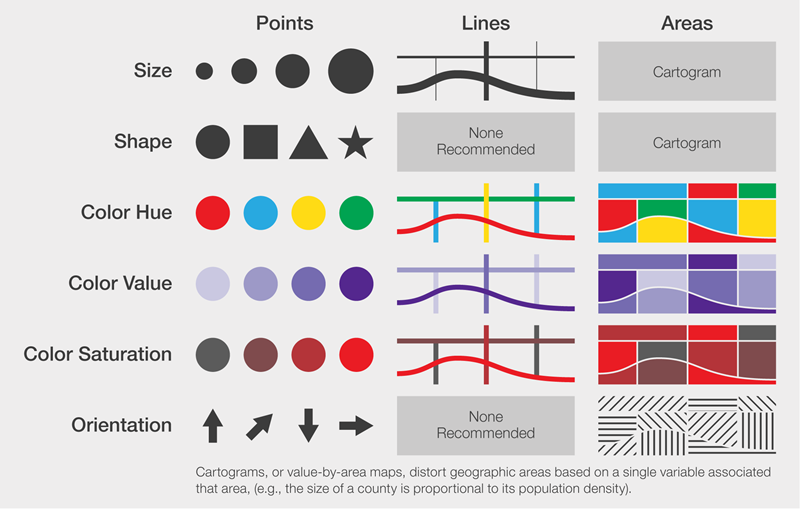
\includegraphics[width=\textwidth]{images/visual-variables.png}
  \caption{Bertin's~\cite{Bertin2010} original visual variables.}\label{fig:theory:visual-variables}
\end{figure}

\subsection{Treemaps}
The visualization of hierarchical data has a long tradition.
The traditional representation of a tree is a rooted, directed graph with the root node at the top.
An everyday use case is a directory tree example of a file system, e.g.\ in file browsers or command line utilities like \texttt{tree} in UNIX based operating systems.
As \textcite{Shneiderman1992} mentions, this visualization becomes increasingly large when displaying more than one node and soon exceeds the entire screen size.
\textcite{Johnson1991} proposes the tree map visualization technique, in which each node is a rectangle whose area is proportional to a specified dimension.
Rectangles contain sub-branches of the node as tiles, thereby expressing hierarchy information.
\begin{figure}[h]
    \centering
    \copyrightbox[b]{%
        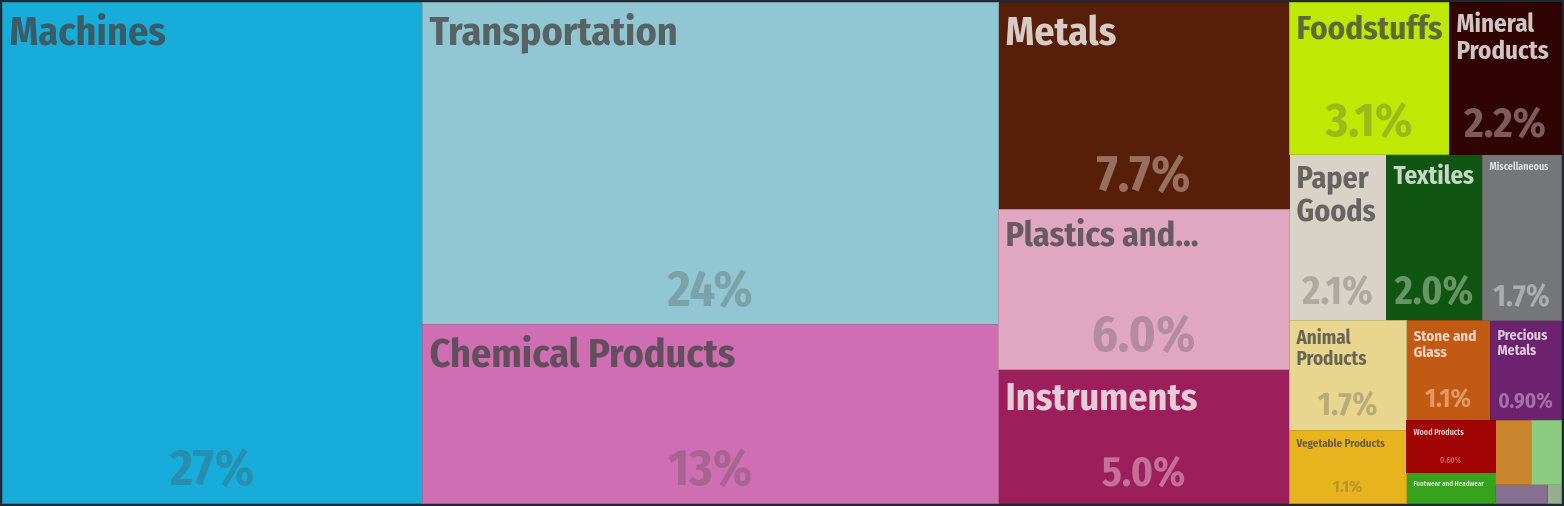
\includegraphics[width=\textwidth]{images/theory/german-exports-1}}{%
        \hfill \ccAttribution{} \ccShareAlike{} Observatory of Economic Complexity~\cite{Macro2017}
    }
    \caption{First hierarchy level of German exports}\label{fig:theory:treemap-german-exports-1}
\end{figure}

\begin{figure}[h]
    \centering
    \copyrightbox[b]{%
        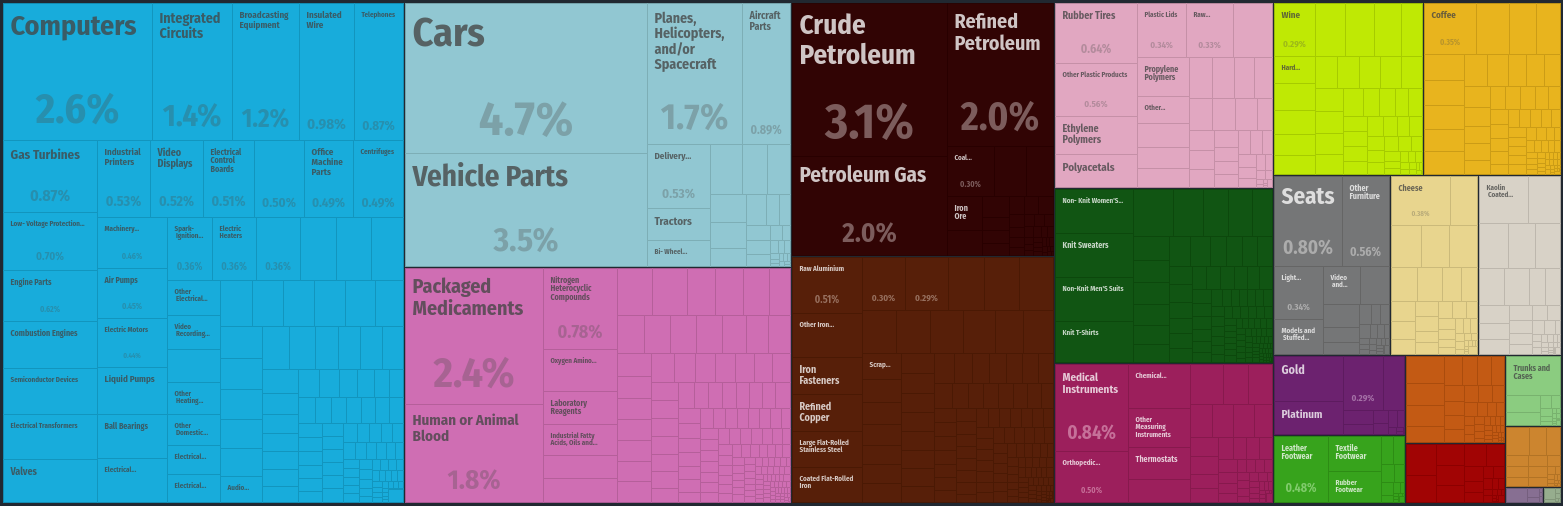
\includegraphics[width=\textwidth]{images/theory/german-exports-2}}{%
        \hfill \ccAttribution{} \ccShareAlike{} Observatory of Economic Complexity~\cite{Macro2017}
    }
    \caption{Second hierarchy level of German exports}\label{fig:theory:treemap-german-exports-2}
\end{figure}
We can see an example of an interactive treemap in Figures~\ref{fig:theory:treemap-german-exports-1} and~\ref{fig:theory:treemap-german-exports-2}.
German exports are divided in generic groups like ``Machines'' and ``Chemical Products'' and include more specific groups like ``Cars'' and ``Packaged Medicaments''.
The level of hiearchy can be selected with a dropdown menu, so only leaf nodes are displayed at a time.
Treemaps are space-filling visualizations, i.e.\ they make 100\% use of the available screen size.

Note that as the order and placement of the nodes depends on the value of their specified dimension, geographical units of data may may be placed separately on the treemap.

\paragraph{\threedTmaps{}} is a concept introduced by \textcite{Bladh2004} in 2004.
The authors transfer the concept of tree maps from two dimensional into three dimensional space.
They introduce StepTree~\cite{Bladh2004}, which is a three dimensional tree map to display a directory layout.
It ``differs from Treemap in that it employs three dimensions by stacking each subdirectory on top of its parent directory.''
3D tree maps are superior to 2D tree maps for tasks with a pronounced topological challenge.
User perform significantly better in interpreting the hierarchical structure.
However, 3D visualizations also introduce some disadvantages as superimposition of objects and a complex view point navigation.

\paragraph{\tmap{}} is a term coined by \textcite{Limberger2016}.
A \tmap{} emphasizes physical constraints of a \threedTmap{}, i.e.\ a \tmap{} has all items attached to the ground.
We can see an example of a \tmap{} in figure~\ref{fig:research:ua_treemap}

\begin{figure}[h]
  \centering
  \copyrightbox[b]{%
    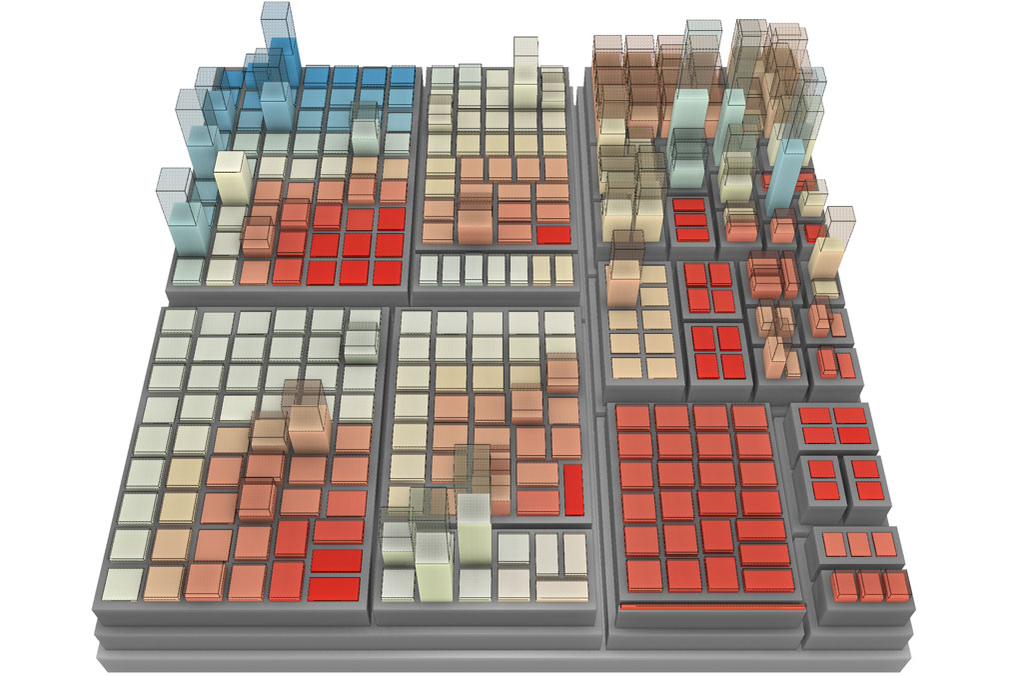
\includegraphics[width=\textwidth]{images/2_5D_treemap_example}}{%
    \hfill \textcopyright{} Hasso-Plattner-Institut\cite{Doellner2017}
  }
  \caption{Example of a \tmap{}}\label{fig:research:ua_treemap}
\end{figure}


\subsection{Geographical Maps}
\todo[inline]{introduction}
\paragraph{Flow maps} place stroked lines on top of a geographic map.
They often display the flow of goods or the migration of people.
As we can see in Figure~\ref{fig:theory:flow-map}, an early example of a flow map is Charles Minard’s depiction of Napoleon’s ill-fated march on Moscow in 1861~\cite{Corbett2001}.
\begin{figure}[h]
  \centering
  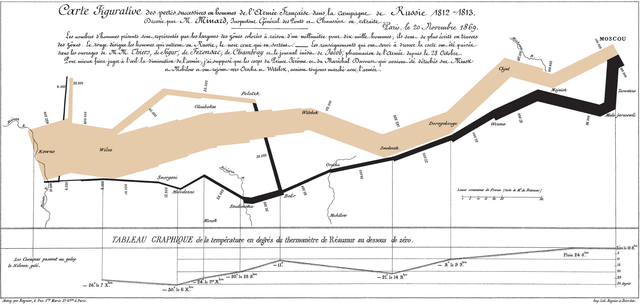
\includegraphics[width=\textwidth]{images/theory/minard}
  \caption{%
    Charles Minard's map of Napoleon's disastrous Russian campaign of 1812.
    Minard managed to represent six values in two graphical dimensions:
    The number of Napoleon's troops, the travelled direction and distance, latitude and longitude relative to specific dates and the temperature.
  }\label{fig:theory:flow-map}
\end{figure}

\paragraph{Chloropleth maps} is a thematic map in which areas are shaded or patterned in proportion to the statistical variable being displayed on the map.
A popular use case is the display of population density or per-capita income.
We can see an example of a choropleth map in figure~\ref{fig:theory:choropleth}, showing the percentage of obese population in the US\@.
Choropleth maps are widely popular and likely to understand them.
They are very helpful when data is attached to enumeration unites like counties, provinces and countries.

\begin{figure}[h]
  \centering
  \copyrightbox[b]{%
    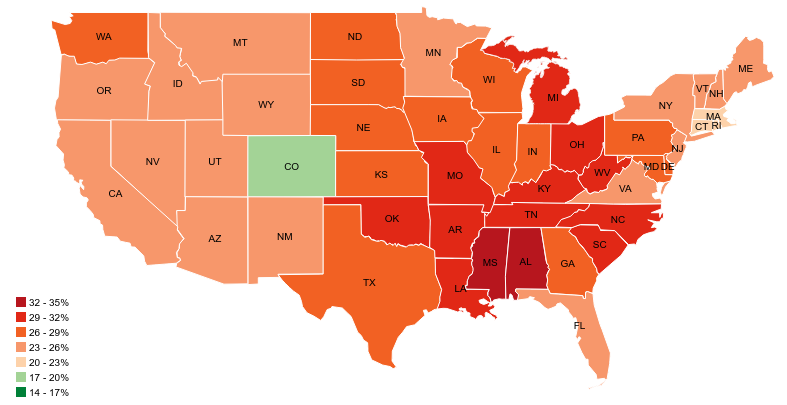
\includegraphics[width=\textwidth]{images/theory/choropleth}}{%
    \hfill National Center for Chronic Disease Prevention and Health Promotion~\cite{NCCDPHP2017}
  }
  \caption{%
    Choropleth Map of Obesity in the United States in 2008.
    Present of population classified as ``obese'' (Body Mass Index in excess of 30), by state.
  }\label{fig:theory:choropleth}
\end{figure}

\paragraph{Graduated Symbol Maps} is a good alternative to a choropleth maps, as it alleviates one of its downsides:
Larger areas may appear more emphasized than smaller ones, thus confounding geographic area with data values.
Instead, symbols are placed over the regions of a map.
As \textcite{Heer2010} point out, these symbols allow for more visal variables to be visualized, i.e.\  symbol size, shape and colour.

\paragraph{Cartograms} are used to encode a data attribute in the size of an area.
For this reason geographic regions in cartograms appear distorted.
A common example is to redraw the size of a country based on the the population or gross domestic product of a country.
Area cartograms may be contiguous or noncontiguous, depending on the applied layout algorithm.

\subsection{Coordinated Multiple Views}
According to \textcite{Roberts2007} \cmvs{} is just ``a specific exploratory visualization technique that enables users to explore their data''.
\cmvs{} are characterized by the fact, that they show multiple views side-by-side.
We can see an example in figure~\ref{fig:research:cmv}.
It displays an on-time performance of airlines, visualized with the ``Crossfilter'' javascript library.
The user can set the borders of an interval with the mouse in each of the views.
The visualization takes the most recent 80 flights from the database that match all given filters.
All visualizations are then updated in real time.
As we can see in the example in figure~\ref{fig:research:cmv} there seems to be a correlation of a long delay with a later time of the day.

\begin{figure}[h]
  \centering
  \copyrightbox[b]{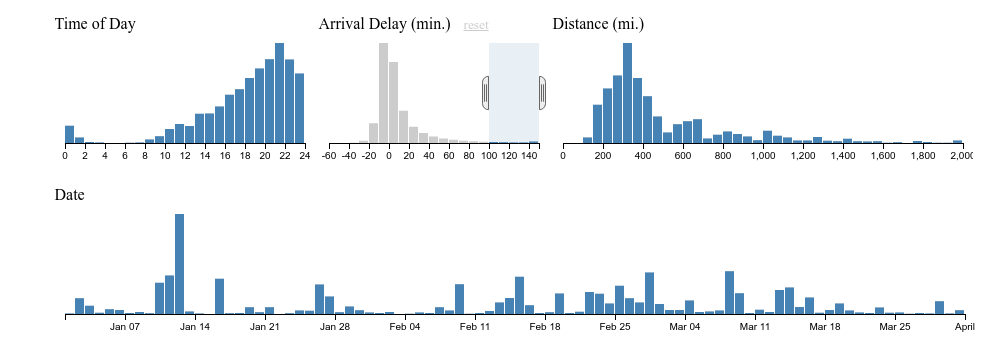
\includegraphics[width=\textwidth]{images/cmv_example}}{\hfill Crossfilter\cite{Bostock2017}}
  \caption{Airline on-time performance: Correlation of time of day with arrival delay. Most recent flight with a delay of more than 100 minutes selected.}\label{fig:research:cmv}
\end{figure}

\paragraph{Brushing and Linking}
Most multiple coordinated views also provide some kind of brushing technique.
``The technique of brushing is the principle approach, where elements are selected (and highlighted) in one display, concurrently the same information in any other linked display is also highlighted.''\cite{Roberts2007}

\clearpage
\section{Related Work}\label{sec:related-work}
According to \textcite{Ho2013} interactions are a crucial part of data visualizations, yet most research in the area of data visualization still focuses on visual representations.
Roughly speaking, research on interaction falls into these groups:
How to categorize interaction techniques?
How to find new interaction techniques and apply those to visualizations?

\todo[inline]{Give a rough overview of this section}
\subsection{Categories}\label{sec:related-work:categories}
\textcite{Shneiderman1996} classifies interactions into these groups:
\begin{enumerate*}[label=(\arabic*)]
  \item
    Gain an \emph{overview} of the entire collection,
  \item
    \emph{zoom} in on items of interest,
  \item
    select an item or group and get \emph{details} when needed,
  \item
    view \emph{relationships} among items,
  \item
    keep a \emph{history} of actions to support undo,
  \item
    allow \emph{extraction} of sub-collections and of the query parameters.
\end{enumerate*}

In 1997 \textcite{Shneiderman1996} classified interactions into these groups:
\begin{enumerate*}[label=(\arabic*)]
  \item
    Gain an \emph{overview} of the entire collection,
  \item
    \emph{zoom} in on items of interest,
  \item
    select an item or group and get \emph{details} when needed,
  \item
    view \emph{relationships} among items,
  \item
    keep a \emph{history} of actions to support undo,
  \item
    allow \emph{extraction} of sub-collections and of the query parameters.
\end{enumerate*}

Two years later, \textcite{Dix1998} identified these categories:
\begin{enumerate*}[label=(\arabic*)]
  \item
    \emph{Highlight and focus} particular subsets of the data,
  \item
    instead of displaying everything simultaneously \emph{access extra information} by drilling down the data,
  \item
    zoom in and out to give an \emph{overview and context},
  \item
    \emph{change parameters} of the \emph{same representation}, e.g.\ another baseline of a stacked bar char,
  \item
    \emph{change representation} of the \emph{same data} by switching the chart type,
  \item
    \emph{link representations} to determine the relationship between items.
\end{enumerate*}

In 2002, \textcite{Keim2002} comes up with the following classification:
\begin{enumerate*}[label=(\arabic*)]
  \item
    Dynamic \emph{projection} to show all combination of data attributes mapped to the axis of a diagram,
  \item
    focus on a smaller subsets by \emph{filtering} out parts of the data,
  \item
    \emph{zoom} into a subset of the data and get a higher level of detail,
  \item
    preserve an overview of the data during drill-down operations is called \emph{distortion}
  \item
    and finally \emph{link and brush} visualizations, to highlight the same data points in multiple visualizations.
\end{enumerate*}

The most recent classification was done in 2007 by \textcite{Yi2007} listing seven categories:
\begin{enumerate*}[label=(\arabic*)]
  \item
    \emph{Select} to mark something as interesting,
  \item
    \emph{explore} to show something else,
  \item
    \emph{reconfigure} to show a different arrangement,
  \item
    \emph{encode} to show a different representation,
  \item
    \emph{abstract/elaborate} show more or less detail,
  \item
    \emph{filter} show something conditionally,
  \item
    \emph{connect} show related items.
\end{enumerate*}

\todo[inline]{The classifications are all redundant! Explain why and choose one classification for later use}
\todo[inline]{Give one example for each category of the chosen classification}

\subsection{Interaction Theory}
\todo[inline]{no section without text}

\paragraph{Space-Time Cube Operations}
is a concept introduced in 2014 by \textcite{Bach2014} to map temporal data into two dimensional visualizations.
Space-time-cubes are used to model two attributes of continuous data with temporal data along a third axis, therefore the name \emph{cube}.
While the transformations are rather static it is also possible to introduce activity into the transformations.
The authors describe user-independent \emph{animations} and user-controlled \emph{interactions}.
E.g.\ a transformation may display a given slice of the cube.
An animation would display one slice at a time and display the next slice every second.
Whereas the interaction would show the slice determined by a user-controlled slider.
Various transformations and their best use in practice are evaluated in this work.
The work focuses on temporal data and otherwise continuous data.
Interactions are not seen as an abstract entity, that need to be agnostic of the underlying data structure and visualization.
The authors admit ``our framework does not provide much guidance for interaction design: the design space for interactive operations has only been partially explored.''\cite[Other limitations, p.~15]{Bach2014}

\paragraph{ITlib\cite{Figueroa2001}} is an architecture and a framework of interaction techniques for virtual reality applications, designed to be extensible and flexible.
New interaction techniques can easily be added and application specific code is seamlessly integrated.
On a low level an interaction technique ``is modeled as a set of filters connected in a small data flow''\cite[Basic concept, p.~2]{Figueroa2001}.
These filters are the smallest process unit in the data flow.
Composed of input and output ports, they communicate with other filters, to receive data input from predecessors and send data output to successors.
The framework specifies and stores the interaction techniques along with its filters, the execution model and the scene in XML documents.
The authors chose XML because it can be parsed easily and they generate code in order to target various virtual reality toolkits and environments.

Even though the system describes interactions in an abstract way, the domain of the framework is clearly the interaction of a human body within a 3D virtual reality.
Certain assumptions are made, including the data model, which is the 3D scene, and human computer interaction devices, like the user's hand or the user's head.
The goal is not to better understand the data, as the data model in this case is the 3D scene, and not statistical data.
Most important, the framework describes interaction techniques for a single viewpoint but not for coordinated multiple views.

\paragraph{Focus+Context Visualization} by \textcite{Bjork1999} is one of the few formalizations of information visualizations.
The authors describe this formalization based on first-level and second-level visualization:
\subparagraph{Visualizations} referred to as $IV$, are triples of a set $[D]$ of underlying data, a visual representation $V$ and $I$ which is the possible interaction or manipulation. 
\begin{equation}
  IV([D], V, I)
\end{equation}
If $I$ affects $[D]$ we can manipulate the underlying data set.
Examples would be changes in a spreadsheet editor, or a change of the start and end date of an appointment in a calendar.
When $V$ is affected by $I$ the user can manipulate $IV$ in order to change the way $[D]$ is represented, e.g.\ choosing a different level of detail as shown in Figures~\ref{fig:theory:treemap-german-exports-1} and~\ref{fig:theory:treemap-german-exports-2}.

\subparagraph{Second-level Visualizations} are information visualizations consecutively applied.
The underlying data set $[D]$ of the previous formula is replaced with some information visualization $IV$, which is compatible with $IV'$.
\begin{equation}
  IV'(IV, V', I')
\end{equation}


Focus+context visualizations are second-level visualizations.
An example given by the authors is the  ``rubbersheet'' visualization, that visually distorts a first-level visualization similar to a magnifier.




\clearpage
\section{Use case}\label{sec:use-case}
\todo[inline]{No section without text}

\subsection{Data Sets}
For our uses cases, we have two different data sets:
One data set consists of a user ranking of public broadcasting in Germany, i.e.\ entities, mostly TV and radio broadcasts, are liked or disliked by people.
This data is public data and can be used by media researchers of broadcasting corporations but also targets media journalists and the general audience.
The other set, called \riso{}, consists of statistical data from various German administrations and is used by the authorities for urban planning and policy strategies.

Both data sets share some characteristics.
The administrative data connects certain features with certain regions of Germany.
As Germany is a federal state, larger regions consist of many other smaller regions.

The second one consists of user data that was collected through a web application called \rufu{}.

\subsubsection{RISO}

The \riso{} data base is used in by local authorities to get insights about governmental KPIs to assist local and regional decision making.
It is a relational database and a part of the data base schema is shown as an ER diagram in figure~\ref{fig:data:riso}.

\begin{figure}[h!]
  \centering
  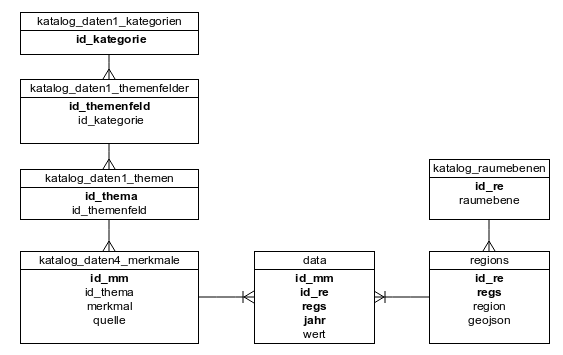
\includegraphics[width=\textwidth]{images/riso}
  \caption{Part of the \riso{} database schema. Primary keys are set in bold.}\label{fig:data:riso}
\end{figure}

The largest table is called \attr{data} with approximately 10,466,600 records, which holds all values along with the survey date.
\paragraph{Features}
This data is connected to a feature table through a foreign key called \attr{id_mm}.
In the feature table we can find the description for every referenced feature, e.g.\ population density, working population in agriculture, education spending.
The \riso{} system groups all features in a 4-level hierarchy:
\begin{enumerate}
  \item
    \attr{katalog_daten_1_kategorien}
  \item
    \attr{katalog_daten_2_themenfelder}
  \item
    \attr{katalog_daten_3_themen}
  \item
    \attr{katalog_daten_4_merkmale}
\end{enumerate}
The actual features table is the last one in the list.
At the lowest level within the hierarchy, this is the largest table with 1234 records.


\paragraph{Regions}
On the other side, the geographical data is stored in the \attr{regions} table.
The geometry data for each region is stored in the \attr{geojson} column and as the name suggests, the data type is a \attr{geojson}.
The foreign keys that connect the tables \attr{data} and \attr{regions} are called \attr{id_re} and \attr{regs}.
Unlike the feature table, the regions are grouped through the \attr{id_re} that indicates the hierarchy level.
So the values of the \attr{id_re} column denominate the level of the hierarchy.
E.g.\ a region with a \attr{id_re} of $1$ is a federal state of Germany, a region with id $13$ is a constituency.
A textual description for the hierarchy level can be found in the \attr{katalog_raumebenen} table in column \attr{raumebene}.
Both column \attr{id_re} and \attr{regs} belong to the primary key of the regions table, so there will never be two regions on the same hierarchy level with the same \attr{regs} id.

\paragraph{Characteristics}
As we can see, the schema of the \riso{} database follows a rather denormalized approach.
The schema does not make a lot of assumptions regarding the input data.
It allows to add data of arbitrary size, features and completeness as long as there is some kind of numerical data associated with some kind of geographical unit.
This approach is suitable for a data base that incorporates data from different sources, as it is the case with the \riso{} data base.


\subsubsection{\rufu{}}
Unlike the \riso{} database, the data base of \rufu{} is used as persistence layer.
For that reason the data base schema follows the requirements of a web application in production.

As outlined in Section~\ref{sec:outline} \rufu{} is an evaluation platform for public broadcasting in Germany.
First, users vote on broadcasts, i.e.\ they decide if they want to support broadcast or if they do not want to support.
As a next step, user can define a weighting by distributing a virtual, monthly budget among the chosen broadcasts.

Figure~\ref{fig:data:rundfunk} shows the data base schema of the application.
A \attr{user} is connected to \attr{broadcast} through a \attr{selection}.
If the \attr{user} supports some a broadcast, the \attr{response} on the given \attr{selection} will be `positive'.
If the \attr{user} does not wish to support a \attr{broadcast}, the \attr{response} will be `neutral'.
The \attr{user} can allocate virtual money to supported broadcasts.
The money will be stored in the column \attr{amount} of the \attr{selection}.
The sum of all amounts for one user will never exceed the virtual budget of 17.50€.

\begin{figure}[h!]
  \centering
  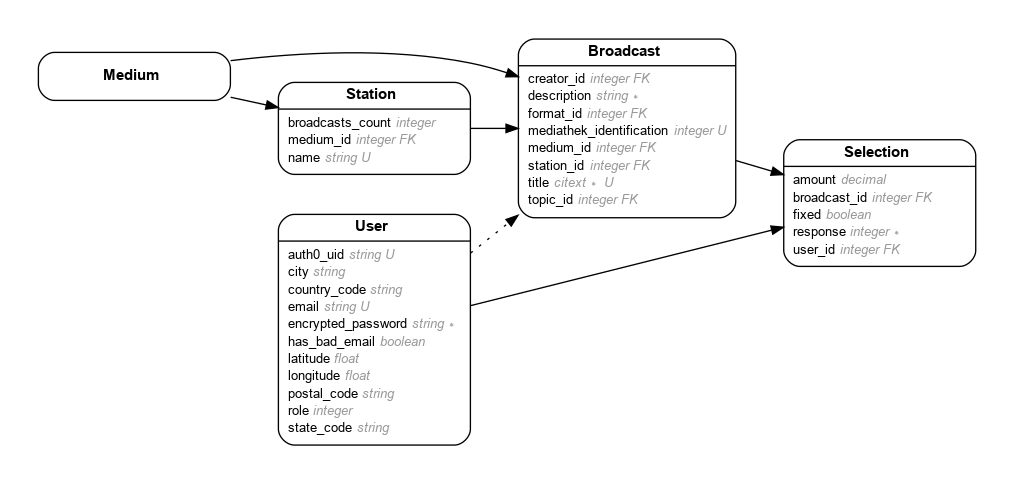
\includegraphics[width=\textwidth]{images/er}
  \caption{Database schema of the \rufu{} app}\label{fig:data:rundfunk}
\end{figure}

\paragraph{Features}
We have both numerical as well as nominal features.
A numerical feature could be the number of supporters from an area in Germany.
A nominal feature could be a list of the most supported broadcasts from an area in Germany.
Numerical and nominal features can be combined, so we could request for every region, a distribution of the desired expenditure for radio, TV, online and other broadcasts.

\paragraph{Regions}
\rufu{} stores the geometry for each region in \attr{geojson} files.
These files hold a \attr{FeatureCollection}.
Every \attr{Feature} is a region, the identifier is stored as a property.
We merge the geometry data with features for every request.
To be precise: We get all the user data, group it by the identifier \attr{state_code} and merge it with the geometry in the \attr{geojson}.

\paragraph{Characteristics}
The data base schema is a result of the specific requirements of the persistence layer.
Changes in the source code may require a migration of the data base schema.

However, we can ask a lot of questions already with common data base queries or standard data analysis tools:
\begin{enumerate}
  \item
    How does the actual support of a broadcast compare to the average support of a broadcast?
  \item
    What are the most popular broadcasts in Berlin?
  \item
    What is the desired ratio of genres of supported broadcasts? How important is education compared to sport?
  \item
    How does the support of a broadcast change over time?
  \item
    According to the user ranking, which broadcasts are similar to each other?
\end{enumerate}


\subsection{Existing Interactions}
We will now classify the implemented interactions of our two applications according to the classification by \textcite{Yi2007} in Section~\ref{sec:related-work:categories}.

\paragraph{In our \visan{}} possible interactions can be categorized into the classes \emph{select}, \emph{explore}, \emph{reconfigure}, \emph{encode} and \emph{filter}.
As seen in figure~\ref{fig:analysis:interaction:existing} the user can \emph{select} one item in the view by clicking on it.
The user can reveal a tooltip showing the item properties by hovering with the mouse on the item, which is another \emph{selection}.
The user can \emph{explore} the map in the usual manner:
If the user drags with the mouse on the map, a panning operation is performed with the viewpoint focused on Germany, i.e.\ the camera moves around like a turntable.
The zoom factor can be changed by scrolling on the canvas of the map.
\emph{Encode} and \emph{reconfigure} techniques are performed through the menu on the left side:
Under the ``features'' tab, the user can \emph{reconfigure} different data sets and the displayed diagram, e.g.\ a tree map visualization based on the geometry shape, cubes or voronoi regions.
The tab ``Dimensions'' allows the user to \emph{encode} properties of a data set to visual attributes, e.g.\ the height, color and texture of an item.
The tab ``Filter'' can be used to reduce the displayed data set along a range of continuous values.
Figure~\ref{fig:analysis:interaction:existing:filter} shows the range of visible values in the left menu.
When the user drags the slider, the items in the map on the right side are updated interactively.

\begin{figure}[h!]
  \centering
  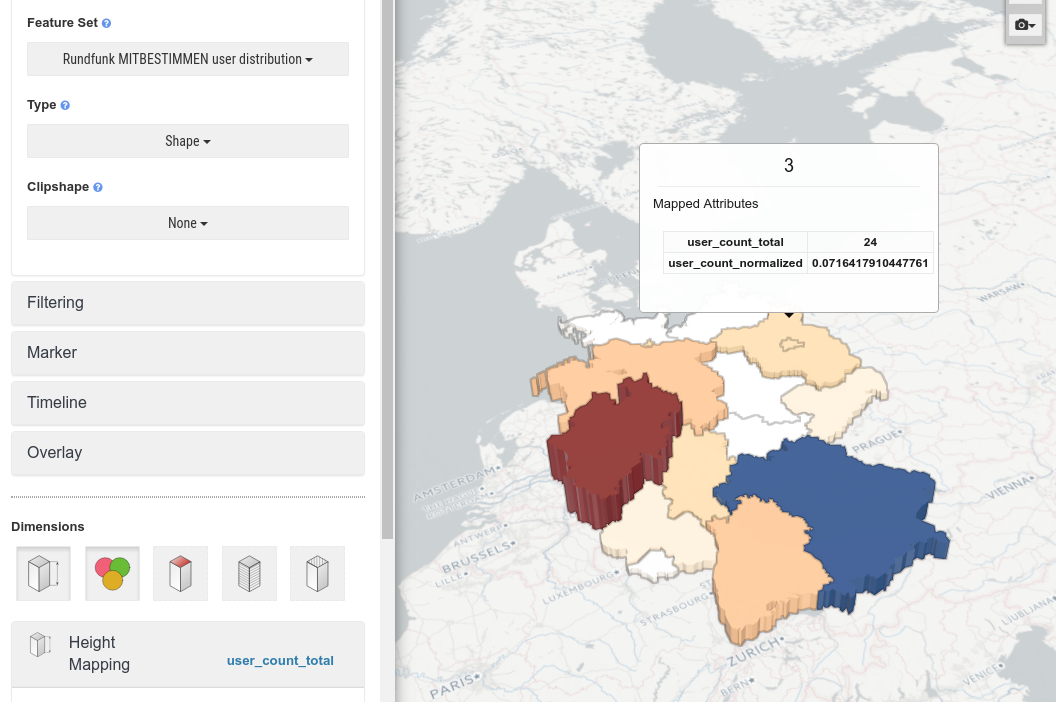
\includegraphics[width=\textwidth]{images/existing-interactions.png}
  \caption{%
    Items can be highlighted with a click, Bavaria is currently highlighted.
    A mouse over reveals a tooltip showing item properties.
    The menu on the left side allows to change the data set and the specific base visualization.
  }\label{fig:analysis:interaction:existing}
\end{figure}

\begin{figure}[h!]
  \centering
  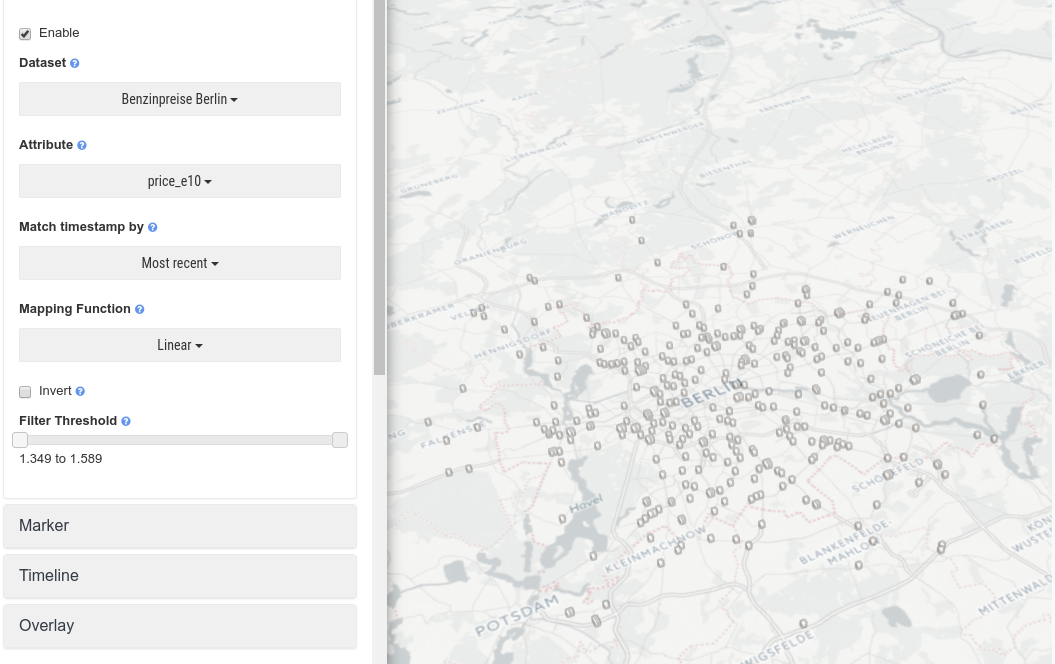
\includegraphics[width=\textwidth]{images/existing-interactions-filter.png}
  \caption{%
    Only gas stations with a price for E10 within 1.349 Euro and 1.589 Euro are displayed in the map
  }\label{fig:analysis:interaction:existing:filter}
\end{figure}

\subsection{Planned Interactions}
We have a focus on coordinated multiple views consisting of a tree map and a geographical map.
Let's have some examples how an interaction between a \tmap{} and a \map{} might work:

    \begin{enumerate}
      \item
        User selects a feature set from the drop down in the menu. This will trigger a \emph{Reconfigure} interaction. A data set consisting of all features and their ids, geometries and metadata is transferred. The receiving components are both the \tmap{} and the \map{} which will rerender the entire visualization.
      \item
        User hovers with a mouse over a polygon in the \map{}. This will trigger a \emph{Select} interaction. The data is a single feature id that will be transferred to the \tmap{}, which will change the color of an box.
      \item
        Rotate or zoom the \tmap{}. This will also rotate or zoom the \map{}. The interaction would fall into \emph{Explore} and the shared information is the orientation of the camera and the zoom level.
      \item
        A click in the \tmap{} will trigger an \emph{Explore} interaction. The data is a single feature id sent to the \map{}. The map will center the viewport on the center of geometry of the respective feature.
      \item
        The user selects many features at once in the \map{} by dragging a rectangle. The ids of all features within the rectangle are sent to the \tmap{}. All features will be highlighted with a different color, which is therefore a \emph{Select} interaction.
      \item
        \emph{Reconfigure} the layouting of the \tmap{} by choosing a different hierarchy level. This increased granularity may lead to an increased granularity in the \map{}, e.g.\ show postal codes instead of federal states. The changed data are additional items, that are nested in the former items.
      \item
        \emph{Encode} the \tmap{} by a different attribute mapping like color, height or texture. If the \map{} has no geometry data that defines the shape of a feature, it can also display a larger point marker.
      \item
        Apply a \emph{Filter} and reduce the data set by choosing only items with metadata beyond a certain treshold. The reduced data leads to a full re-render of all data visualizations. The message contains the updated item list
  \item
    Show a \emph{Connect} by highlighting boxes of the same subtree in the \tmap{}. The respective connected items would be highlighted in the \map{} as well. Here the data is a relation between items.
    \end{enumerate}
\todo[inline]{What are the key interactions in our use case?}


\clearpage
\section{Analysis}\label{sec:analysis}
In this section, we list several interaction examples in singular views as well as in multiple views.
We list the expected data structure of each visualization and the respective dependent and independent visual variables according to~\cite{Bertin2010}.
In addition we classify each interaction according to \textcite{Yi2007}.
Finally, we describe the relevant subject of the interaction.
I.e.\ what would be exchanged, if the interaction should be mirrored in an entirely different visualization on the underlying data set.

The goal of this procedure is to abstract and deduce the essential characteristics of any interaction, to pave the way for a formalized language of \cmvs{}.

\subsection{Singular Visualization Interactions}\label{sec:analysis:examples}

The data visualization catalogue by Severino Ribecca list many of the most used data visualizations\cite{VisualizationCatalogue2017}.
Let's pick some of those and derive a number of possible interactions.

%\begin{tabular}{l l l l}
    %Comparisons & Proportions & Relationships & Hierarchy \\
    %Concepts & Location & Part-to-a-whole & Distribution \\
    %How things work & Processes \& methods & Movement or flow & Patterns \\
    %Range & Data over time & Analysing text & Reference tool \\
%\end{tabular}


\paragraph{Line diagrams}
\begin{figure}
  \begin{center}
    \subfloat[Line diagram]{{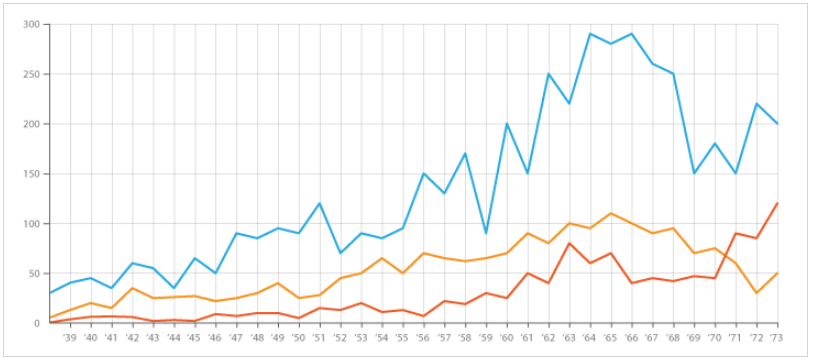
\includegraphics[width=0.4\textwidth]{images/chartTypes/line-diagram.png} }}%
    \qquad
  \end{center}
  \caption{Line charts are used to display trends}\label{fig:concept:chart-types:line-diagrams}
\end{figure}

Line diagrams are multiple sets of data, displayed along the x-axis.
They are used to display quantitative value over a continuous interval or time span.
It is possible to highlight an entire series of data or just a feature within that series.

\conceptTable{Tabular data, many data sets as series.}{Position, orientation, texture.}{Color, shape, size.}

\begin{figure}
    \begin{center}
        \caption{Interactions for line charts}%
        \label{fig:concept:chart-types:line-diagrams:interactions}
        {\small
            \begin{tabulary}{\textwidth}{ll}
                \bf Select & Highlight a data point (id of data point) \\
                \bf Select & Highlight a data series (id of data series) \\
                \bf Encode & Change colours of data series (data series \rightarrow\ colour) \\
                \bf Filter & Restrict interval on x-axis (filter function of data attribute) \\
                \bf Filter & Hide a data series (id of data series) \\
            \end{tabulary}
        }
    \end{center}
\end{figure}



\paragraph{Bar charts and multiset bar charts}

\begin{figure}
  \begin{center}
    \subfloat[Bar chart]{{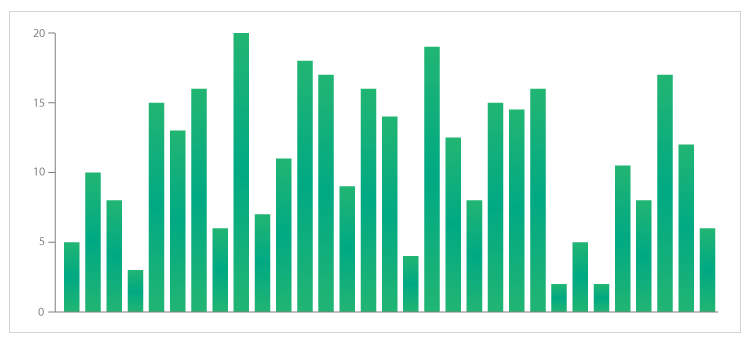
\includegraphics[width=0.4\textwidth]{images/chartTypes/bar-chart.png} }}%
    \qquad
    \subfloat[Multiset bar chart]{{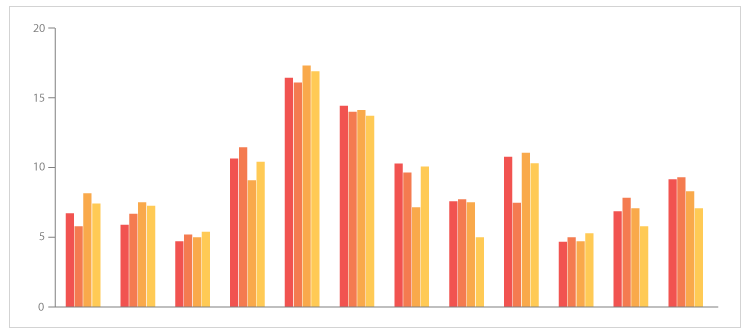
\includegraphics[width=0.4\textwidth]{images/chartTypes/multiset-bar-chart.png} }}%
  \end{center}
  \caption{A multiset bar charts is a variation of a bar chart}\label{fig:concept:chart-types:bar-charts}
\end{figure}

Bar charts and multiset bar charts show one or many attributes per feature along an axis.
They have in common that they encode the data attribute into the height of the eponymous bars.
Colors might be used to better distinuish between the different data attributes.
Features can be arbitrarily ordered along the axis, although multiset bar charts group features along a series of categories.

Therefore, bar charts need to be initialized with the set of features and their values as well as the groups of features for the multiset bar chart.
The supplied colours would colour each feature in a group in turn.
The set of possible ineractions include the highlighting of features, the reordering of features and a change in encoding of colour values.

\conceptTable{Tabular data, many data sets as series}{Size, orientation.}{Position, colour, shape, texture.}

\begin{figure}
    \begin{center}
        \caption{Interactions for bar charts}\label{fig:concept:chart-types:bar-charts:interactions}
        {\small
            \begin{tabulary}{\textwidth}{ll}
                \bf Select & Highlight a bar (id of data point) \\
                \bf Encode & Change colours of data series (colours \rightarrow{} data series) \\
                \bf Reconfigure & Sort by attribute (data attribute) \\
                \bf Reconfigure & Drag bars to reorder data series (ordered list of ids of data points) \\
                \bf Filter & Hide a data series (id of data series) \\
            \end{tabulary}
        }
    \end{center}
\end{figure}


\begin{figure}
  \centering
    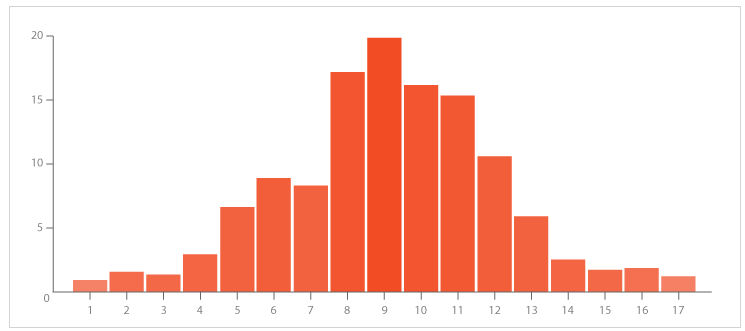
\includegraphics[width=0.4\textwidth]{images/chartTypes/histogram.png}%
    \label{fig:concept:chart-types:histograms}
    \caption{A histogram is a bar chart over a continuous interval}%
\end{figure}

Histograms visualise the distribution of data over a continuous interval or certain time period.
A special type is the population pyramid, which is a pair of back-to-back histograms, one for each sex.
The difference of histograms to bar charts lies in the type of data itself, not the representation.
Therefore these charts need to be initialized with the same data and the same interactions can be applied.

\conceptTable{Tabular data, many data sets as series}{Size, orientation, position.}{Color, shape, texture.}

\paragraph{Bubble charts and scatter plots}

\begin{figure}
  \centering
    \subfloat[Bubble chart]{{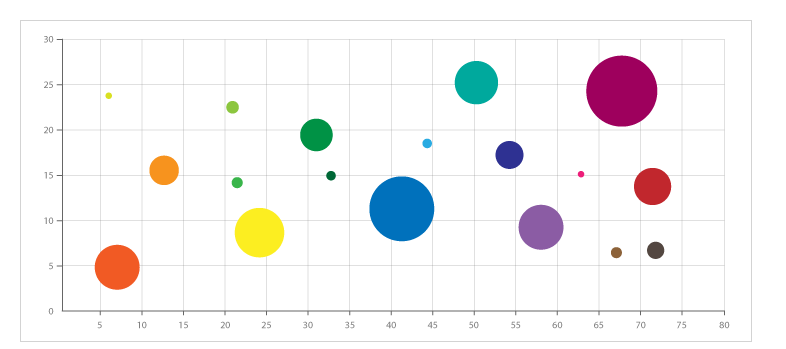
\includegraphics[width=0.4\textwidth]{images/chartTypes/bubble-chart.png} }}%
    \qquad
    \subfloat[Scatter plot]{{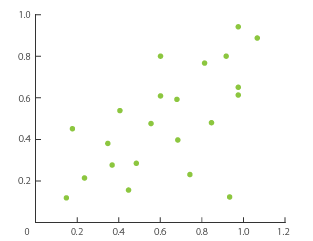
\includegraphics[width=0.4\textwidth]{images/chartTypes/scatter-plot.png} }}%
    \caption{Bubble charts and scatter plots are similar regarding interactions}%
    \label{fig:concept:chart-types:bubble-chart}
\end{figure}

Bubble charts are popular choices to display a distribution of features.
The chart is initialized with coordinates for each feature, a colour and a size in case of a bubble charts.
Possible interactions include the highlighting of features, a different colour encoding, a reconfiguration to map another attribute to size.
Bubble charts may show only a window of the available data and allow to zoom in, zoom out or move the window along the axes.

\conceptTable{Tabular data, single data set with x- and y-coordinates}{Size, position.}{Color, shape, texture, orientation.}

\begin{figure}
    \begin{center}
        \caption{Interactions for bubble charts}%
        \label{fig:concept:chart-types:bubble-chart:interactions}
        {\small
            \begin{tabulary}{\textwidth}{ll}
                \bf Select & Highlight a bubble (id of data point) \\
                \bf Explore & Zoom in, zoom out (width and height of window) \\
                \bf Explore & Move viewport position (x- and y-coordinates of viewport) \\
                \bf Encode & Change mapping of colour to category (data series \rightarrow\ colour) \\
                \bf Encode & Change colour function (function value \rightarrow\ colour) \\
                \bf Encode & Change data attribute to colour (data attribute) \\
                \bf Encode & Change data attribute to size \\
                \bf Reconfigure & Sort by attribute (data attribute) \\
                \bf Reconfigure & Drag bars to reorder data series (ordered list of ids of data points) \\
                \bf Filter & Hide a data series (id of data series) \\
            \end{tabulary}
        }
    \end{center}
\end{figure}

\paragraph{Stacked bar charts}

\begin{figure}
  \centering
    \subfloat[Stacked bar chart]{{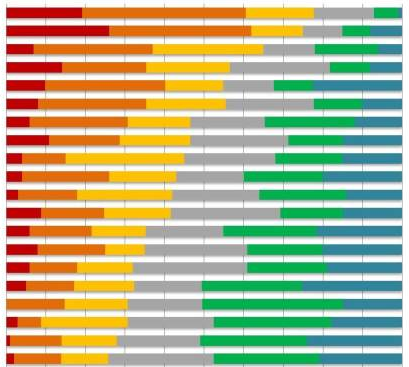
\includegraphics[width=0.3\textwidth]{images/chartTypes/stacked-bar-without-baseline.png} }}%
    \qquad
    \subfloat[Stacked bar chart with baseline]{{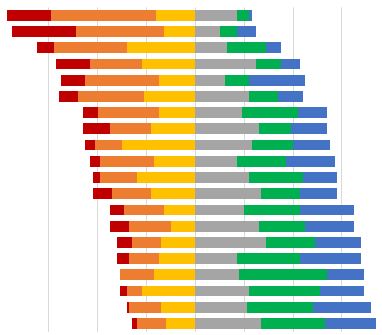
\includegraphics[width=0.3\textwidth]{images/chartTypes/stacked-bar-with-baseline.png} }}%
    \caption{Stacked bar charts can be ordered along a baseline or stretch to 100\% width to show the percentage-of-the-whole of each group}%
    \label{fig:concept:chart-types:stacked-bar-chart}
\end{figure}
\begin{figure}
  \centering
    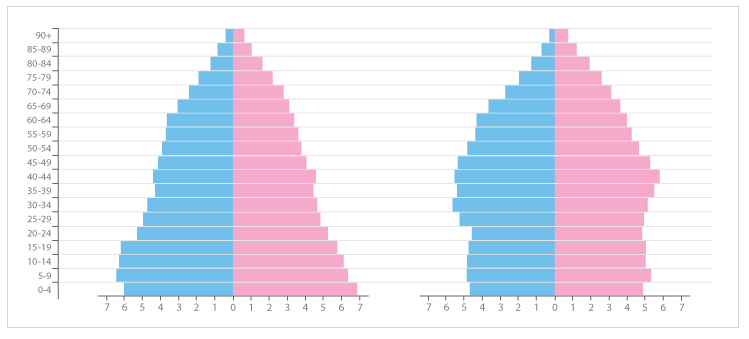
\includegraphics[width=0.4\textwidth]{images/chartTypes/population-pyramid.png}%
    \label{fig:concept:chart-types:population-pyramid}
    \caption{A population pyramid can be modeled as a stacked bar chart}%
\end{figure}

Unlike a multi-set bar graph which displays their bars side-by-side, stacked bar graphs segment their bars of multiple datasets on top of each other.
A baseline, as shown in figure~\ref{fig:concept:chart-types:stacked-bar-chart} might be modeled as two back-to-back multi-set bar graphs. A reordering would e.g.\ move one data set from the left side to the right side.
Possible interactions include the highlighting of a feature, a change of color mapping, reordering of the baseline.

\begin{figure}
    \begin{center}
        \caption{Interactions for stacked bar charts}%
        \label{fig:concept:chart-types:stacked-bar-chart:interactions}
        {\small
            \begin{tabulary}{\textwidth}{ll}
                \bf Select & Highlight a bar (id of data point) \\
                \bf Encode & Change mapping of category to colour (data series \rightarrow\ colour) \\
                \bf Reconfigure & Sort by attribute (data attribute) \\
                \bf Reconfigure & Reorder Y axis (ordered list of ids of data points) \\
                \bf Reconfigure & Sort stacking order by attribute (data attribute) \\
                \bf Reconfigure & Specify the stacking order data series (ordered list of ids of data series) \\
                \bf Reconfigure & Specify a negative data series (list of ids of data series) \\
                \bf Filter & Hide a data series (id of data series) \\
            \end{tabulary}
        }
    \end{center}
\end{figure}

\conceptTable{Tabular data, multiple date sets as series}{Size, shape, orientation.}{Color, position, texture.}

\paragraph{Hierarchical visualizations}

\begin{figure}
  \centering
    \subfloat[Tree map]{{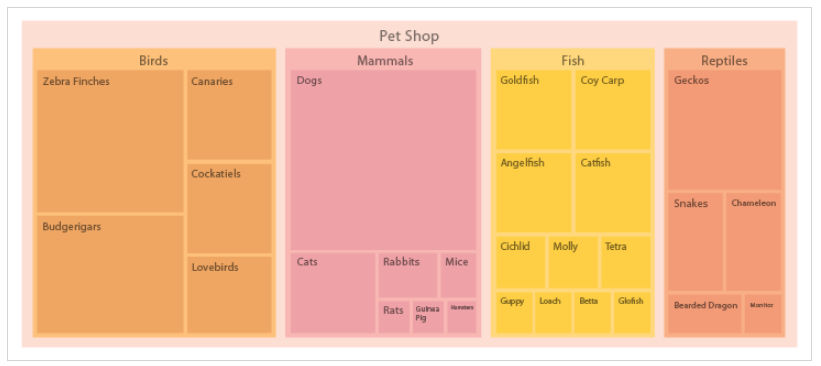
\includegraphics[width=0.4\textwidth]{images/chartTypes/treemap.png} }}%
    \qquad
    \subfloat[Sunburst diagram]{{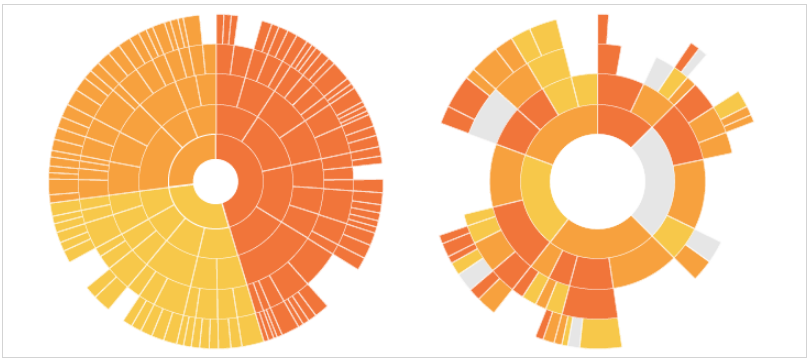
\includegraphics[width=0.4\textwidth]{images/chartTypes/sunburst.png} }}%
    \caption{Tree maps and sunburst diagrams are ideal to show hierarchies}%
    \label{fig:concept:chart-types:hierarchies}
\end{figure}

Treemaps are great to show hierarchical data without ever exceeding the availabe screen.
Each feature is a assigned a rectangle according to a layouting algorithm.
Unlike a tree map a hiearchical ring diagram or sunburst diagram shows each level of the tree as a series of rings.

Therefore, both tree map and ring diagram need the feature set as a tree, with each node having a data attribute for layouting. Every node may be assigned a color.
As we are describing hierarchies, the maximal depth of tree may be increased or decreased.
Again, interactions could include a highlighting of features and a change of color encoding.
Both visualizations may show only a subtree.
E.g.\ a click on a box in the treemap opens another treemap focused on the subtree.
Similarly a click on a slice of the ring would surround the most external ring with the children of the feature.

\conceptTable{Tree, each feature has a value for layouting.}{Position, Size, shape, orientation.}{Color, texture.}

\begin{figure}
    \begin{center}
        \caption{Interactions for hierarchical visualizations}%
        \label{fig:concept:chart-types:hierarchies:interactions}
        {\small
            \begin{tabulary}{\textwidth}{ll}
                \bf Select & Highlight a feature (id of data point) \\
                \bf Explore & Use another node as root of the visible tree (id of data point) \\
                \bf Encode & Change mapping of category to colour (data series \rightarrow\ colour) \\
                \bf Reconfigure & Change data attribute used for layouting (data attribute) \\
                \bf Reconfigure & Sort by attribute (data attribute) \\
                \bf Reconfigure & Specify order (ordered list of ids of data points) \\
                \bf Abstract/Elaborate & Specify maximum depth of visible tree (number of levels) \\
            \end{tabulary}
        }
    \end{center}
\end{figure}

\paragraph{Geographical Data}

\begin{figure}
  \centering
    \subfloat[Choropleth map]{{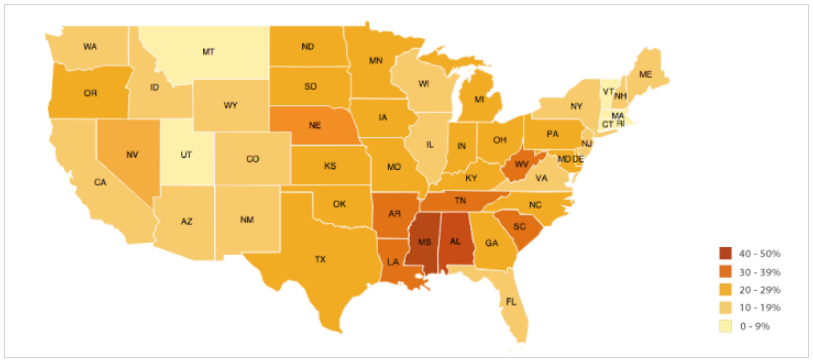
\includegraphics[width=0.4\textwidth]{images/chartTypes/choropleth-map.png} }}%
    \qquad
    \subfloat[Flow map]{{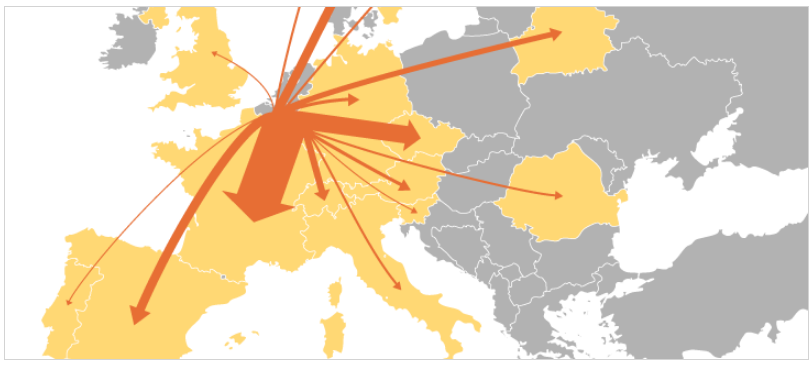
\includegraphics[width=0.4\textwidth]{images/chartTypes/flow-map.png} }}%
    \caption{Choropleth maps focus on a density while flow maps show a migration of data}%
    \label{fig:analysis:chart-types:geographical}
\end{figure}

Choropleth maps and flow maps are specialized diagrams focused on geographical data.
Size, position and shape of a feature is defined by the geometry data of a feature.
In choropleth maps the color of each feature is based on a data attribute.
Flow maps may display connections between features, a data value defining the size of each arrow.

\conceptTable{Graph data with edges, each feature has geometry data.}{Position, Size, shape, orientation.}{Color, texture.}

\begin{figure}
    \begin{center}
        \caption{Interactions for geographical visualizations}%
        \label{fig:concept:chart-types:geographical:interactions}
        {\small
            \begin{tabulary}{\textwidth}{ll}
                \bf Select & Highlight a feature (id of data point) \\
                \bf Explore & Move viewport (latitude and longitude of viewport)\\
                \bf Explore & Zoom in, zoom out (zoom factor) \\
                \bf Encode & Change shape of marker (data id \rightarrow\ shape) \\
                \bf Encode & Change mapping of category to colour (data series \rightarrow\ colour) \\
                \bf Encode & Change colour function (value \rightarrow\ colour) \\
                \bf Encode & Change data attribute used for colour (data attribute) \\
                \bf Connect & Show relations of a feature (id of data point)  \\
                \bf Abstract/Elaborate & Change granularity of displayed regions (number of levels) \\
            \end{tabulary}
        }
    \end{center}
\end{figure}

\paragraph{Activity diagrams}
\begin{figure}
  \centering
    \subfloat[Calendar]{{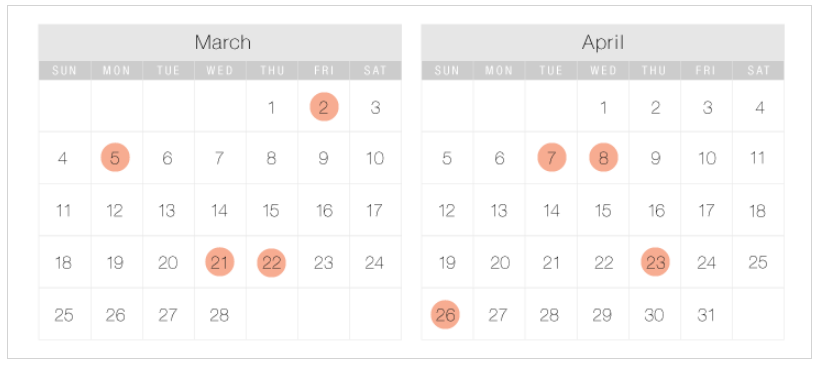
\includegraphics[width=0.4\textwidth]{images/chartTypes/calendar.png} }}%
    \qquad
    \subfloat[Gantt chart]{{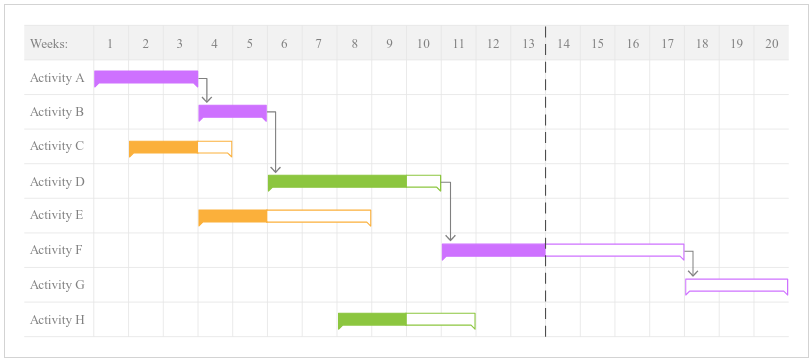
\includegraphics[width=0.4\textwidth]{images/chartTypes/gantt-chart.png} }}%
    \caption{Similar to a calendar, a gantt chart shows activities and the progress along a time line}%
    \label{fig:concept:chart-types:temporal}
\end{figure}

In activity diagrams, each feature is represented as a rectangle, with the duration of the activity mapped to size and position.
Calendars and gantt charts could not only read the data from the data source, but also add new features to the data set or update metadata of a feature, e.g.\ the progress of the activity.

\conceptTable{Temporal data, each feature has a time interval.}{Position, Size, orientation.}{Color, shape, texture.}

\begin{figure}
    \begin{center}
        \caption{Interactions for temporal visualizations}%
        \label{fig:concept:chart-types:temporal:interactions}
        {\small
            \begin{tabulary}{\textwidth}{ll}
                \bf Select & Highlight a feature (id of data point) \\
                \bf Explore & Show a different period of dates (start and end datetime)\\
                \bf Explore & Show a different time interval (start and end hour)\\
                \bf Encode & Change color of categories or activities (data series \rightarrow\ colour) \\
                \bf Encode & Change data attribute used for colour (data attribute) \\
                \bf Filter & Remove a calendar or a category (id of data series) \\
            \end{tabulary}
        }
    \end{center}
\end{figure}

\subsection{Multiple View Interactions}\label{sec:analysis:examples}

\paragraph{Detail view}
\begin{figure}
  \centering
  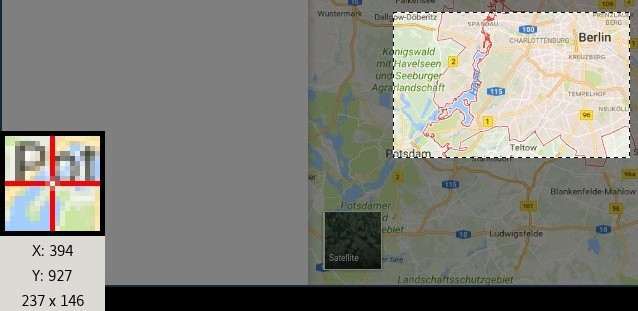
\includegraphics[width=0.4\textwidth]{images/chartTypes/multi/detail-view}
  \caption{The screenshot-tool ``shutter'' shows a magnified detail view of the area around the mouse cursor in the lower right corner of the screen}\label{fig:concept:chart-types:detail}
\end{figure}

\clearpage
\section{Concept}\label{sec:concept}
\todo[inline]{No section without text}

\subsection{Common interface}

Having a central controller be responsible for the entire coordination of views can lead to maintainability issues.
If a new interaction needs to be implemented, a change in the multiview controller is required.
This low flexibility leads to higher development costs and is therefore not desirable.

The question here is:
Is there a way to anticipate what kind of data any interaction might affect?
What kind of visual changes are possible at all in which types of visualization?
What is the expected data structure for which types of visualization?
Are there any other shared concepts in all data visualizations?

If there are shared concepts, we might be able to model common interface for all types of visualizations.
Multiple views would only need to implement to adapter to this interface.
With this interface we would reduce the currently $N*N$ transformations down to $N$ adapters and reduce the overall development costs.

\subsection{Trigger, effect and interaction type}

Let's have a closer look what steps a coordinated interaction actually performs.
First of all, different visualizations have different capabilities and different degrees of freedom how to interact with and display the data.
We choose a \emph{highlight} interaction in our \tmap{} as an example.
The interaction is started by a low level mouse click event inside the visualization.
We call this a \emph{trigger.}
The change of the color of a box is perceived by the user.
We call this change an \emph{effect.}

Both trigger and effect have a certain meaning for the user.
In this case, the user is selecting a particular feature in order to highlight it.

We want to coordinate this interaction in multiple views.
In order to do so, we need to extract the abstract meaning, the \emph{type} of an interaction.
Other visualizations could behave in a way that represents the same type of interaction.
Thus, the type of the interaction needs to be exchanged in different views.
Also, it needs to be exchanged, what the interaction affects, i.e\ the \emph{subject} of the interaction.

We will face some issues in coordinating the types to other views, because:
\begin{enumerate}
    \item
        The effect of the interaction cannot be applied to other views.
    \item
        The relevant interaction type is ambiguous.
    \item
        The low level event that is used as a trigger for the interaction is different.
\end{enumerate}
An example for the first case is to express a highlight interaction with a change of colour.
E.g.\ a bubble chart might encode a certain data attribute to the colour of a bubble.
Therefore the colour cannot be changed.
Another example for the first case:
The data sets of a bar chart could be ordered according to a user interaction.
But the ordering cannot be reflected with a change of position in a scatter plot, as the position is tied to a data attribute.

For the second case, we can see an ambiguity of interaction type if we look at line diagrams and a bar charts.
A user might click on a line in the line diagram to highlight the \emph{entire series of data}.
But in a bar chart a user would click on a bar to select a \emph{feature} of a series, not the entire series of data.

A geographical map might use the mouse drag event to move the viewpoint, which would be an \emph{explore} interaction.
But the drag of a mouse could be used in an activity diagram to change metadata, like the start and end time of an activity.

It is possible to describe interactions in any type of data visualization by looking on the \emph{trigger}, the \emph{effect} and the exchanged \emph{interaction type}.
Coordinating interactions across multiple views then means to make a reasonable choice of \emph{trigger} and \emph{effect} for every view and then define what data is included in the \emph{interaction type}.


\subsubsection{Free visual variables allow for interaction effects}

In order to communicate the interaction to the user, the effect of the visualization must be communicated back to the user by a visual change.
Data visualizations have \emph{dependent} and \emph{independent} visual variables, see~\ref{sec:theory:visual-variables}.
Dependent variables are those that are tied to a data attribute.
These constrained visual attributes are unavailable while independent visual variables are therefore available to be used for a visual feedback of an interaction.

\subsubsection{List events as candidates for interaction triggers}

Interaction can be triggered by any input of a human-computer-interaction device, like the keyboard or the mouse.
Because users are in the habit of expecting certain interactions to be triggered from certain events, we also have constraints here.
E.g.\ the viewpoint in geographical maps is moved by mouse drag events and the zoom level is controlled by the mouse wheel.
So we should not use those already occupied events as triggers for our coordinated interactions.
Nevertheless, consistency in user interfaces is crucial for great user experience, because users can reuse the learned knowledge.
Therefore, we need to list all availabe events as candidates and connect them to our interactions in a preferrably consistent manner.

On the other hand, we might have special controls in visualizations, in order to change the encoding.
E.g.\ a \tmap{} shows a menu where the user can define how attributes are mapped to visual variables.

\subsubsection{Specify the interaction type}

The types of a interaction can be manifold.
\emph{Select}, \emph{Explore}, and \emph{Filter} interactions affect data items.
For that reason, the types of the interaction is the type of interaction plus the identifier of the affected data item.
A highlighting of a bar in a bar chart would consist of the interaction type \emph{select} and the respective \emph{feature id}.
But sometimes, groups of data are selected, like an entire series of data or a subtree in case of hierarchical data.

\emph{\emph{Reconfigure}} and \emph{encode} interactions do not affect data items but the data visualization itself.
The types of these interaction can be arbitrary, e.g.\ an ordered list of feature ids to define the order or a data object that models the mapping of data attributes to visual variables.

\emph{Abstract/elaborate} and \emph{connect} interactions are special interactions which expect a certain type of data.
Increasing the level of detail expects a tree of data with the level of detail determining the maximum depth of the visualized tree.
Showing connections between features expects a graph of data, with edges between features and properties on these edges.


\subsection{Interaction subject space}\label{sec:concept:space}
To account for the various data structures, we use an abstract data model that is powerful enough to include tabular, hierarchical and relational data.
You can see a class diagram in figure~\ref{fig:concept:meta-data-structure}.

The \emph{entity} class is used to model the smallest distinguishable unit.
All entities can be identified and retrieved via the \emph{id}.
An entity is defined to be any object that can have data attached as \emph{attribute}.

While entities describe what an object \emph{is}, an \emph{attribute} describes what it \emph{has}.

An entity can have arbitrary many attributes and each value can be accessed by the name of the attribute.
So if you want to get the \emph{latitude} value of an entity, you can retrieve the value with a call to the named attribute \emph{latitude}.

Entities can also be \emph{series} of other entities.
A series contains an ordered list of contained entities.
As series can also contain other series, so we can model a hierarchy relation.

There is always one particular series without a parent.
This is the root node of the hierarchy.
If we just want to display tabular data, we just have one or two levels of hierarchy.
E.g.\ one level of hierarchy for a histogram and two levels of hierarchy for a stacked bar chart.

Other relations than hierarchical relations can be modeled as a \emph{relation} entity.
It represents a directed edge in a graph and must have incoming and outgoing entity.
Since every \emph{relation} is an \emph{entity} as well, we can add \emph{attributes} to the relation.
These attributes may describe e.g.\ the weight of an edge in a flow map.


\begin{figure}[h!]
  \centering
  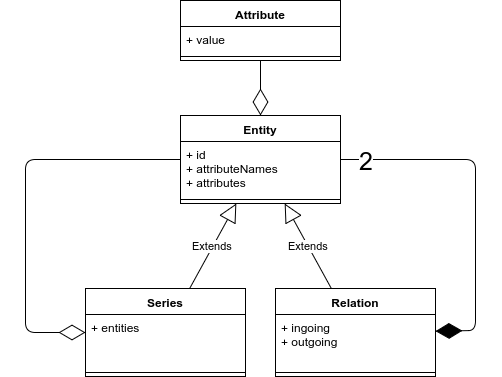
\includegraphics[width=0.5\textwidth]{images/meta-data-structure.png}
  \caption{%
    A data structure for tabular, hierarchical and relational data
  }\label{fig:concept:meta-data-structure}
\end{figure}

\subsection{Interaction types}\label{sec:concept:types}

It turns out that we can describe the types of an interaction as a mathematical function.
These functions operates on the ids of \emph{entities}, \emph{series}, and \emph{relations} or their respective \emph{attributes}.
The name of the function is the \emph{type} of the interaction and the function domain being the \emph{subject} of the interaction.
Thus, we can describe interaction through a change of its semantic but we ignore implementation details of specific visualizations.


These function are derived from specific interactions of the examples in Section~\ref{sec:analysis:examples}.
Domain and codomain of these functions refer to the objects defined in the data model in Section~\ref{sec:concept:space}.
To declare the functions explicitly, we define a couple of sets:
\begin{enumerate}
    \item
        $ \mathbb{E} : \mathbb{E} \subseteq \mathbb{N} $

        The set of ids of all entities in our subject space.
    \item
        $ \mathbb{A} : \mathbb{A} \subseteq \mathbb{\sum^*} $

        The set of names of all attributes in our subject space.
    \item
        $ \mathbb{D} $

        The set of possible data values of any attribute in our subject space. Those values could be e.g.\ numbers, strings, ordinal values, dates or geometries.
    \item
        $ \mathbb{C}: \{ (r,g,b) \in \mathbb{C} | r \in \mathbb{R} \land g \in \mathbb{R} \land b \in \mathbb{R} \}$

        The set of colours, we assume a triple of $R$, $G$ and $B$ values.
    \item
        $ \mathbb{V} $

        The set of visual variables position, size, orientation, texture, colour and shape, as described in Section~\ref{sec:theory:visual-variables}.
        Elements of this set include the name for $x-axis$ and $y-axis$ as well as the name of shapes.
        Thus, an \emph{encoding} interaction can change the mapping of a data attribute to another coordinate axis.
\end{enumerate}

The following is a list of functions describing the types based on the aforementioned sets:
\begin{enumerate}
    \item
        $ Highlight: \varnothing \rightarrow \mathcal{P}(\mathbb{E})$

        A $ Highlight $ is a function without arguments returning a subset of highlighted entities.
    \item
        $ FilterById: \varnothing \rightarrow \mathcal{P}(\mathbb{E}) $

        The $FilterById$ function takes no arguments and returns a subset of entities that are used as input for the visualization.
    \item
        $ FilterByValue: \mathbb{D^*} \rightarrow \{ \bot, \top \} $

        The $FilterByValue$ function takes an ordered list of data values and returns whether or not the associated entity should be part of the visualization input.
    \item
        $ FilterAttributes: \varnothing \rightarrow \mathbb{A^*} $

        The $FilterByAttributes$ returns an ordered list of attributes names.
        Retrieving the values of an entity in order produces the input that can be used as input for the $ FilterByValue $ function.
    \item
        $ Focus: \varnothing \rightarrow \mathbb{E} $

        The $ Focus $ function returns a single id of the entity that should be in the center of the viewpoint.
        Different visualizations can have different interpretations of the semantic:
        A geographical map will move the viewpoint position on the geometric center of the focused entity.
        Hierarchical visualizations, e.g.\  tree maps or sunburst maps, may choose the focused entity to be the root node of the currently displayed subtree.
    \item
        $ Extent: \varnothing \rightarrow \mathcal{P}(\mathbb{E}) $

        This function returns a subset of entities that must be within the current boundaries of the diagram window.
        Again, different visualizations can have different interpretations of the semantic:
        In scatter plots and geographical visualizations the set may be used to implicitly derive the zoom level.
        It can also be used to implicitly derive the maximum depth of the currently visible subtree in a tree map.
    \item
        $ ColourById: \mathbb{I} \rightarrow \mathbb{C} $

        A colour function assigns each entity, data series or relation to a color.
    \item
        $ ColourByValue: \mathbb{D} \rightarrow \mathbb{C} $

        A colour function assigns a continuous value to a color.
        This function can be used by e.g.\ choropleth maps for the background color of regions.
    \item
        $ ColourAttributes: \varnothing \rightarrow \mathbb{A^*} $

        The ordered list of names of attributes used as input for the $ ColourByValue $ function.
    \item
        $ Reorder\rightarrow \mathbb{E^*} $

        The $Reorder$ function defines how a subset of entities should be ordered.
        Note that not the entire collection of entities need to be ordered.
        This sequence will be used in bar charts to order bars along the x-axis or stacked bar charts, to order the stacking of data series.
    \item
        $ Sort: \big( \mathbb{D^*} \times \mathbb{D^*} \big) \rightarrow \mathbb{R} $

        This sort function will return a continuous value based on an arbitrary long list of pairs of data values.
        It's an implicit order function based on one or many data attributes and returns a negative value if the first element is orderd before the second element.
    \item
        $ SortAttributes: \varnothing \rightarrow \mathbb{A^*} $

        The ordered list of names of attributes which will be used as input for the $Sort$ function.
    \item
        $ ReorderAttributes: \varnothing \rightarrow \mathbb{A^*} $

        This ordered list of attributes define in which order visualizations display many coordinate axes.
        E.g.\ a parallel plot can reorder the attributes along the x-axis.
    \item
        $ Encode: \mathbb{A} \rightarrow \mathbb{V} $

        The $Encode$ function can be used to change any mapping of attribute to any visual variable.
        E.g.\ bar charts can change the attribute mapped to the \emph{height} of bars.
        Histograms and scatter plots can change the name attribute that is mapped along the \emph{x-axis}.
        Bubble charts can encode a different data attribute in the \emph{area} of the bubbles.
        A specialized version of this function may return the attribute that is used for the layout algorithm in tree maps. 
\end{enumerate}

Let's have some examples how these functions can be applied on coordinated interactions:

A user clicks on a bar in a bar chart and this feature then changes its background colour.
To coordinate the highlighting, the bar chart visualization replaces the \emph{Highlight} function.
The function now returns the id of the entity of the feature with the new background colour.

When a region in a geographical map is clicked, the new \emph{Focus} function will return the id of the clicked entity.
A coordinated tree map next to the geographical map now shows a subtree with the focused entity as root node.

If many attributes are chosen from a dropdown menu and some thresholds are specified with a slider, both the \emph{FilterAttributes} and the \emph{FilterByValues} functions are changed.
The \emph{FilterAttributes} will return the ordered list of chosen attributes of the dropdown menu.
The updated \emph{FilterByValues} function will now expect a new argument list, based on $ FilterAttributes $.
It then yields either true or false based on the values of these attributes.

\subsection{Coordination of interactions}

In Section~\ref{sec:concept:types} we discussed how we can describe the types of the interaction.
While a type describes the interaction itself and what \emph{subject} it operates on, a type does not describe the actual \emph{coordination} of views.
E.g.\ what action in one view should lead to what kind of changes in what other views?
In addition to the coordination, we need a pattern to exchange messages \cmvs{}.

We regard the messages exchanged between views as a change of those interaction types defined in~\ref{sec:concept:types}
Figure~\ref{fig:concept:trigger-effect} gives a rough overview on our coordination model.
\begin{figure}[h!]
  \centering
  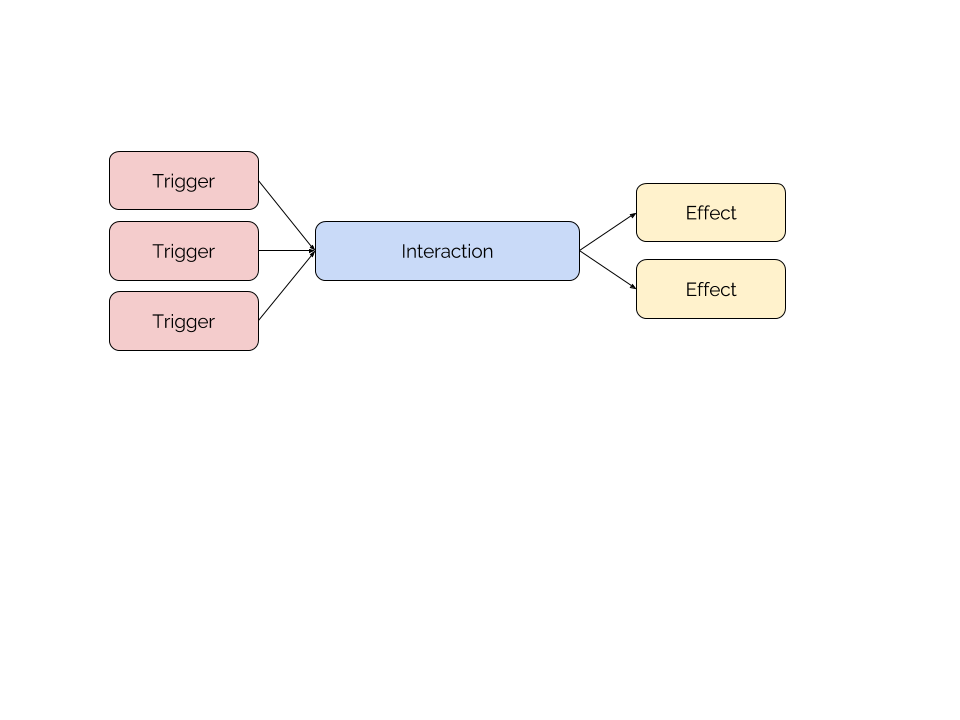
\includegraphics[width=\textwidth]{images/trigger-effect.png}
  \caption{Schema of message flow in \cmvs{}}\label{fig:concept:trigger-effect}
\end{figure}
We introduce two new terms, \emph{trigger} and \emph{effect}.

A trigger is e.g.\ a mouse interaction, like hover or click.
This low-level action is an implementation detail and therefore tied to the specific visualization.

In order to be perceivable by the user, the interaction must have some visual effect.
A feature of the visualization is changed, e.g.\ a colour of a bar in a bar chart.
The choice of the visual effect to express the interaction is an implementation detail as well.

Sometimes a visualization may not be able to interpret an interaction.
E.g.\ a bar chart can re-arrange the bars along the x-axis in case of a \emph{Reconfigure} interaction.
But a scatter plot constrains x- and y-coordinates of an entity on a certain data attribute.
Therefore, not only the \emph{trigger} and \emph{effect} is implementation specific, but also the handling of the interaction itself.

Every visualization decides on its own, how to react to a certain interaction.
That leads us to distinguishable, named interactions.
Every view can subscribe to certain interactions and receive messages in form of changed interaction types.
In order trigger an interaction, the visualization simply publishes to the named interaction.

This pattern is known as the \emph{Publish-subscribe pattern} and widely used in message queues.
The term \emph{interaction} in our case is equivalent to the term \emph{channel} or \emph{topic} commonly used in message queues.


\clearpage
\section{Implementation}

This section describes the implementation details for the described concepts.
We start with a list of to be implemented features.
Next, we describe the architecture of the software and why we chose this architecture.
What requirements and considerations lead to this particular architecture.


\subsection{Implemented interactions}

In the course of this thesis we want to implement the following interactions:
\begin{itemize}
  \item
    \emph{Select}: The user clicks on a building or region in a geographical map and all affected properties in the \tmap{} will be highlighted.
  \item
    \emph{Explore}: The user clicks on a block in the \tmap{} and the viewpoint in the geographical map will be centered on relevant area.
  \item
    \emph{Abstract/Elaborate}: The user selects a different granularity in the geographical map (e.g.\ postal code regions instead of federal states) and the change is reflected in the \tmap{}.
  \item
    \emph{Filter}: The user double-clicks on a region in a geographical map and the \tmap{} will be based on data of only that region.
\end{itemize}

\subsection{Observer pattern}
\todo[inline]{Explain observer pattern}
\begin{figure}[h!]
  \centering
  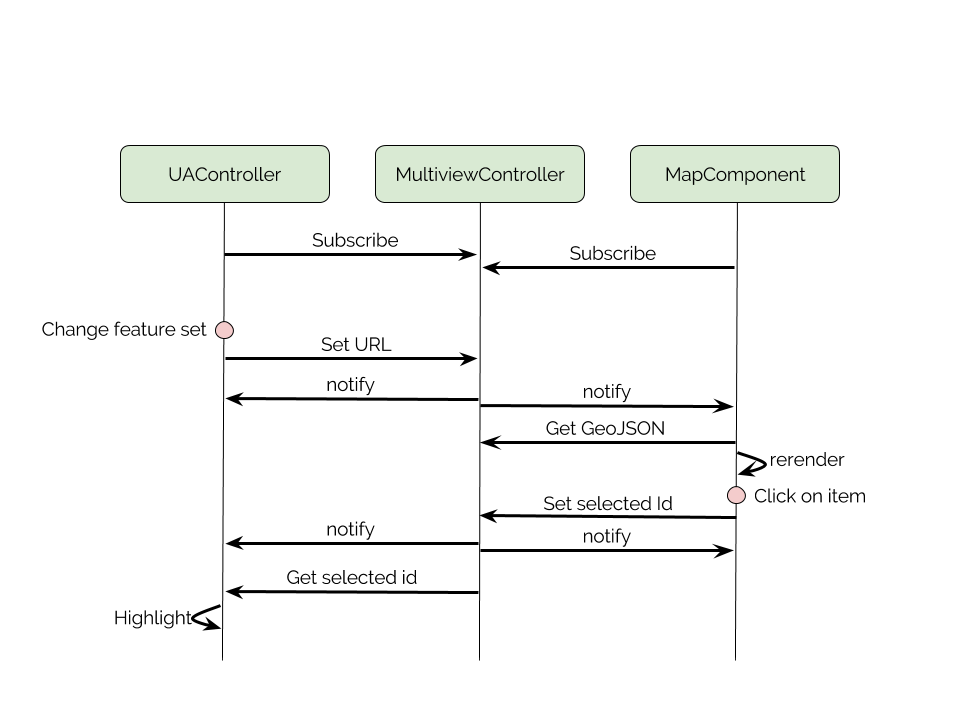
\includegraphics[width=\textwidth]{images/sequence-diagram.png}
  \caption{%
    The sequence diagram shows the notification of different components.
  The user first chooses a feature set and hovers over a polygon in the geographical map.
  }\label{fig:implementation:sequence-diagram}
\end{figure}


Figure~\ref{fig:implementation:sequence-diagram} shows how \cmvs{} can be automatically updated even if the environment lacks a native update-mechanism.
We use the observer pattern:
The root of our views is an observable implementation of the common interface described in section\ref{sec:concept}.
If one of the views updates the view state, it will send the necessary information to the observable.
The observable will then broadcast the change to all it's observers.


\paragraph{Publisher subscriber}
In our particular case we apply a special form of the observer pattern, the so called ``Publish-subscribe'' pattern\cite{Eugster2003}.
Publish-subsribe is a messaging pattern which is widely used in message queues.
In this scenario, senders of messages simply categorize their messages which will be consumed by subscribers of the category.
The scenario has very low coupling, publishers do not even need to know the existence of subscribers.

\todo[inline]{How can multiview subscribe to the multiview controller}

\subsection{Component pattern}
State-of-the-art javascript frameworks like ReactJS and EmberJS follow the component pattern for the architecture of a single page web application.
The component pattern imposes a hierarchical structure on a website.
Each component is responsible for a task and may contain other components.
The components are joined at the root node of the page.

This pattern is very applicable to \cmvs{}.
The different views of \cmvs{} share state, i.e.\ the feature, that is currently highlighted or the applied filter on the data.
So the views are components and their closest common ancestor is the \cmv{} itself, controlling state and passing user interaction down to it's children.

\begin{figure}[h!]
  \centering
  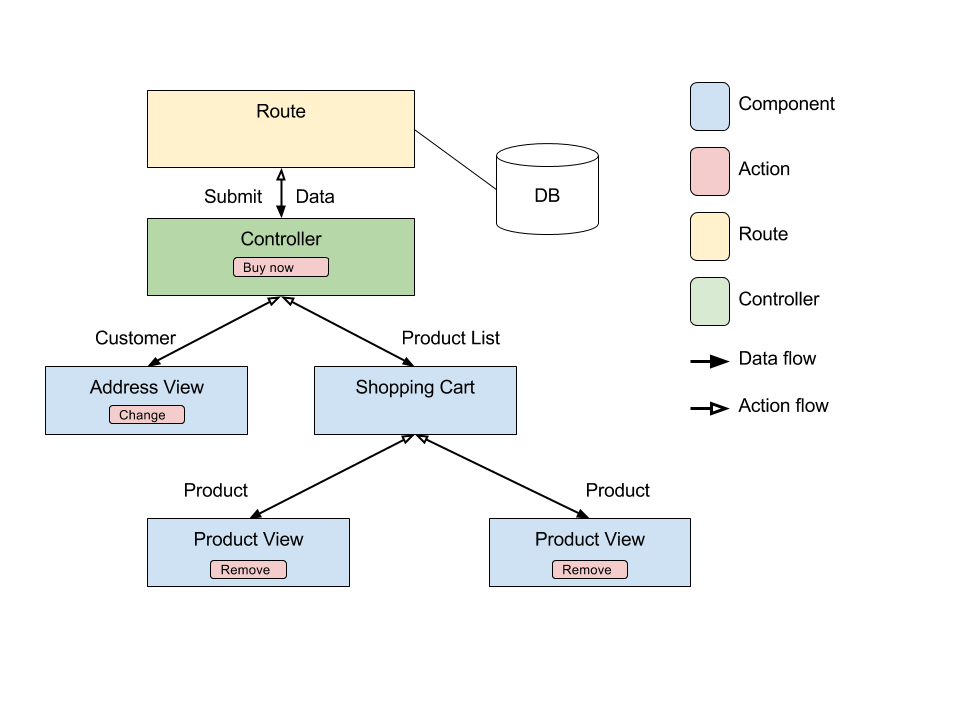
\includegraphics[width=\textwidth]{images/data-down-actions-up.png}
  \caption{%
    Implementation of the component pattern in EmberJS\@.
    The example shows a page of a webshop.
    The customer is about to order the items in the shopping cart.
  }\label{fig:implementation:data-down-actions-up}
\end{figure}

\paragraph{Actions up --- Data down}

Version 2.0 of Ember introduced a common phrase how to use this pattern effectively: ``Data down, actions up''\cite{Emberigniter2017}
In the domain of \cmvs{} actions would mean user interactions, e.g.\ a click on a feature.
The action will notify the controlling \cmv{} component.
Actions may change data, and the changes will be passed to to all dependen views.
These views are then rerendered.

Examples for the kind of data that might trigger a rerendering of a view:
\begin{itemize}
  \item
    The selected feature or a list of selected features
  \item
    A list of thresholds for certain features as a filter
\end{itemize}

\subsection{Web components W3C specification}

Web components is a recent standard of the W3C\cite{W3C2017} to bring component-based software engineering to the world wide web.
They look perfectly suited to be used in \cmvs{}.
However the attributes of web components are string based.
If arbitrary javascript objects need to be passed into the web component it is suggested to use one of the common javascript frameworks that allow for data binding.

\subsection{Frontend framework comparison}

We evaluated three javascript frontend frameworks for our application: \emph{GlimmerJS}, \emph{Google Polymer} and \emph{ReactJS}.
Figure~\ref{fig:implementation:frontend-frameworks} shows the pros and cons of each framework for our use case.

GlimmerJS is the rendering enginge of EmberJS\cite{Ember2017}.
In 2017 it was released as a standalone framework.
Applications written in GlimmerJS can be exported as web components.
These web components can be included in any website, which makes GlimmerJS a reasonable choice to build high-quality widgets for user interfaces.
GlimmerJS also uses handlebars\cite{Handlebars2017}, a user-friendly templating language.
The downside of GlimmerJS is the current lack of documentation and immaturity due to the recent first release this year.

Another popular framework to build web components is Google's Polymer library\cite{Polymer2017}.
With 18,469 stars on Github it is the most popular framework for web components at the time of writing.
Polymer has a large community and comprehensive documentation and therefore more suitable than GlimmerJS for our task.

Unfortunately, the web component standard does not specify how arbitrary Javascript objects can be passed to web components.
This raises some problems in legacy apps:
Usually, legacy apps are written in plain javascript without the use of a component-based frontend framework.
Any part of the code may call any other part of the code, leading to the dreaded ``spaghetti code''.
Refactoring the existing app requires the framework to have a reliable way of communication with the legacy parts.
E.g.\ parts of the legacy code call the backend in order to load data.
This data needs to be passed to the compponents of the user interface.
Web components do not have a designated interface
Because of that, libraries like Polymer come back on proprietary solutions.
But those proprietary solutions defeat the main advantageof developing against a standard, as it is unclear how components may interact with each other.

Lifting the constraint to implement against web components, we finally decided to go for ReactJS\cite{React2017}.
ReactJS does not have the ability to export web components.
It has, in return, an ascertained way of integrating the framework into a legacy app built with jQuery.
Along with its major advantage of easy integration, it has a striving community, heaps of documentation and tutorials and is well tested.

All of these reasons make us choose ReactJS for the task of coordinating multiple views in our existing \visan{}.


\todo[inline]{Pros/cons of GlimmerJS, Polymer, React}


\begin{figure}[h!]
  \centering
  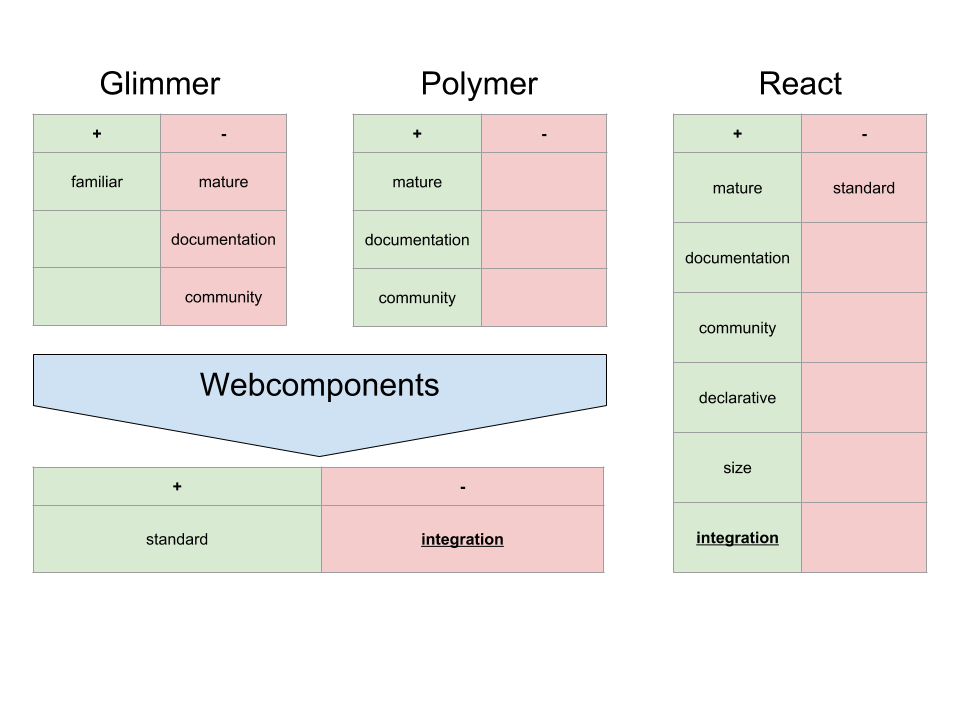
\includegraphics[width=\textwidth]{images/frontend-frameworks.png}
  \caption{Comparison of frontend frameworks}\label{fig:implementation:frontend-frameworks}
\end{figure}

\subsection{Observer pattern and component pattern in \cmvs{}}
Figure~\ref{fig:implementation:both-patterns} shows the final result.
We try to put as much code as possible under the root node of ReactJS\@.
By that we eliminate the amount of custom updating implementation.
The root node of the DOM-tree of our react application is connected with the existing app through the common interface.
Both urban analytics controller and the multiview map component will observe changes to the common interface.
Also sub-components may communicate with the common interface.


\begin{figure}[h!]
  \centering
  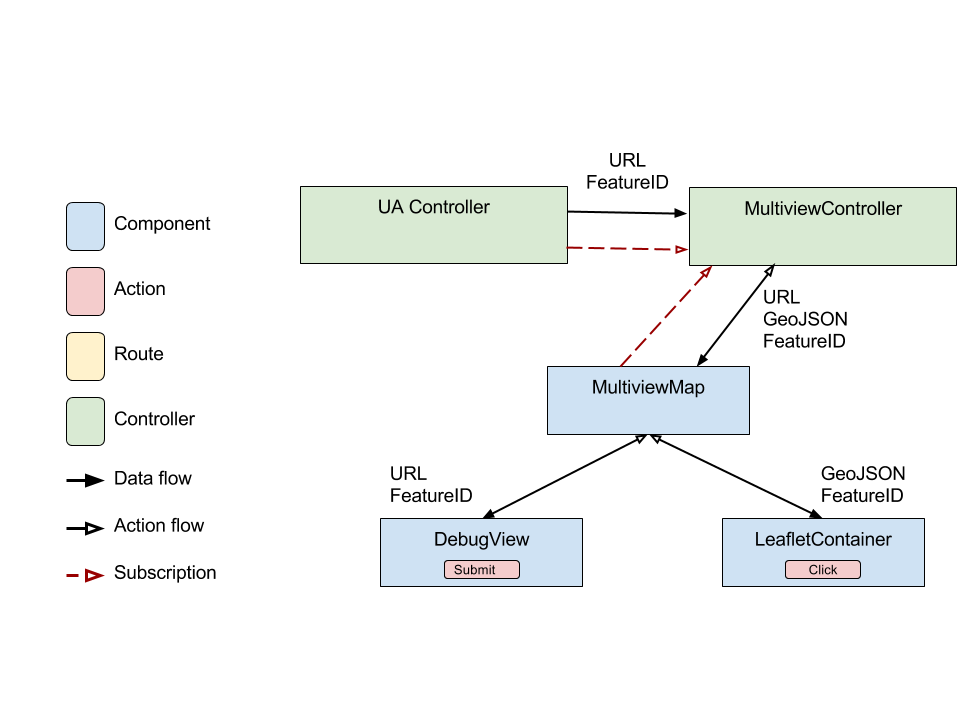
\includegraphics[width=\textwidth]{images/both-patterns-implemented.png}
  \caption{%
    Both observer pattern and component pattern applied in the field of \cmvs{}
  }\label{fig:implementation:both-patterns}
\end{figure}


\subsection{GeoJSON}

An example of aggregated user data merged with geometry data can be seen in listing~\ref{lst:geojson:example}.
\lstinputlisting[language=JavaScript, label={lst:geojson:example}, caption={Geojson example}]{listings/example.geojson}

We can use this data as input for our common \visan{}, e.g.\ figure~\ref{fig:implementation:user_distribution} shows the user distribution of \rufu{}.

\begin{figure}[h!]
  \centering
  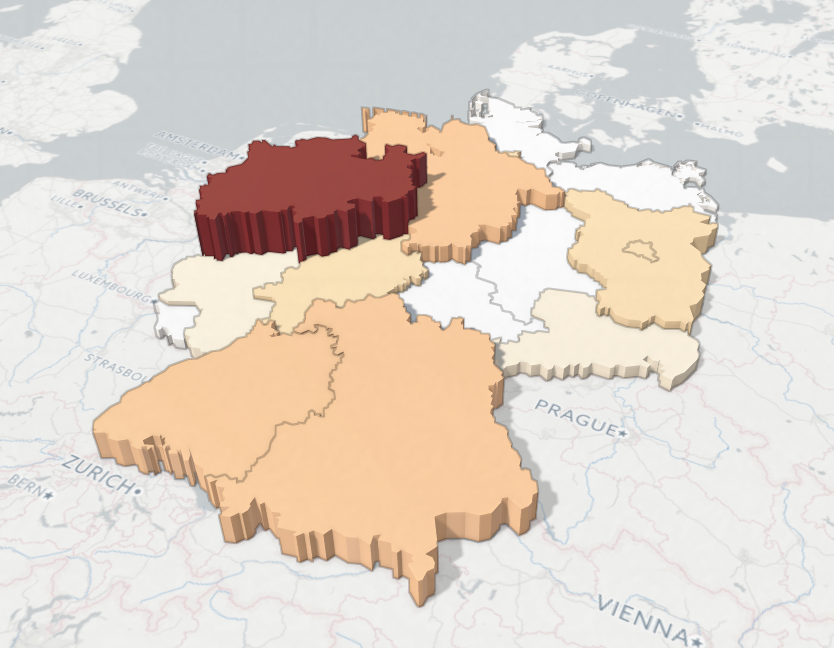
\includegraphics[width=\textwidth]{images/ua_example.png}
  \caption{%
    User distribution of \rufu{} across German federal states
  }\label{fig:implementation:user_distribution}
\end{figure}


\clearpage

\section{Evaluation}
\todo[inline]{How and what can we evaluate?}
\todo[inline]{The performance?}
\todo[inline]{The flexibility?}

\section{Conclusion}
\todo[inline]{Did we achieve our goals?}
\todo[inline]{Is the concept sane in regarding the implementation?}

\section{Future Work}
\todo[inline]{List stuff which was not accomplished in this master thesis}



\clearpage

\printbibliography{}
\end{document}



%\subsubsection{Use case specific problems}
%There is striking discrepancy of intentions between available metrics and the programme mandate of public broadcasting.
%TV ratings are produced by a group of 5000 representative homes equipped with a special TV box, while Radio ratings are carried out by phone surveys over the course of a year.
%Although created differently they share the same intention, i.e.\ to sell advertisements.
%
%We suspect that public broadcasting suffers from an overfitting problem:
%Since broadcasters have usage data only, they focus too much on people who still listen to the radio and watch TV.
%Young people especially show a decreasing interest in conventional mass media which has been shown in surveys.
%Public broadcasting fails in that respect that everybody has to pay and thus has a right to get access to information.

%In many cases, insights based on visualization techniques like \cmvs{} are used by experts for strategic decision-making.
%Thus, many advanced data visualizations techniques are made exclusively for professionals.
%
%On the other hand, data visualizations widely popular:
%Data journalism is one of the emerging fields in journalism.
%Facts and figures are the strongest evidence for opinionated journalistic reports.
%Not even a football match can do without a number based analysis.
%
%We believe that advanced data visualization techniques can be adopted and used in both an informative and strategic way by professionals as well as lay people.



% We use data visualizations in the context of the expenditure of public broadcasting fees in Germany.
% Since the year 2013 these fees are compulsory for every home in Germany and as a consequence, broadcasting receives €8,000,000,000 annually.
% Yet it is subject to little or no public feedback, ranking, or even debate on what constitutes value or quality.
% There is neither transparency on how the fees are spent nor a public feedback on how the fees should be spent.
%
% We see a great potential, a win-win situation to be precise, because both payers of the broadcasting fees and broadcasters themselves can benefit from each other.
% As of 2013 there is no legal opt-out anymore and people have a strong interest to say how their fees should be spent.
% Broadcasters on the other hand can evaluate their program based on the interests delivered by the users.
% This reciprocal relationship would create a public feedback for payers and a better program for broadcasters.
%
% This problem is perfectly suitable to be tackled with data visualizations.
% \todo[inline]{Explain why data visualization are good for communication}

%Our use case is creating a tool to publicly evaluate public broadcasting in Germany.

%Public broadcasting has a long history in all of Europe.
%Especially after the experiences of the Third Reich, freedom of the press and freedom of broadcasting in particular was defined in the German constitution, the basic law.
%Article 5 not only ensures the press to be free of censorship.
%It is interpreted in such a way that it guarantees broadcasting to exist and be politically and economically independent.
%It is remarkably in many ways:
%First, mass media are recognised to be a basic prerequisite for formation of opinion of the general public.
%Second, the state fosters free access to information, ie. Open Knowledge.

%Despite this highly positive ideal, reality looks somewhat different.
%Public broadcasting in Germany receives €8,000,000,000 (eight billion euros) annually, yet it is subject to little or no public feedback, ranking, or even debate on what constitutes value or quality.
%Since 2013, there is no legal opt-out for German citizen anymore.
%Every home in Germany has to pay for broadcasting whether or not the people actually use it.
%This has created numerous constitutional complaints and approximately 2 million homes in Germany refuse to pay, even it is virtually illegal to do so.

